
%%% Uncomment for slide version
\documentclass[xcolor=dvipsnames]{beamer}
\setbeameroption{hide notes} % Only slides

%%% Uncomment for handout version
%\documentclass[handout]{beamer}
%\setbeameroption{show notes on second screen=right} % Both

\usepackage{enumitem}
\usepackage{listings}
\usepackage{adjustbox} % To incorporate code into Latex
\usepackage{multirow} % To merge multiple rows  in a table
\usepackage{soul} % To put in strikethrough text
\usepackage{array}
\usepackage{makecell}

\setbeamertemplate{note page}{\pagecolor{white}\insertnote}
\setbeamertemplate{footline}{}
\usetheme[progressbar=frametitle]{moloch}% modern fork of the metropolis theme
\setbeamercolor{background canvas}{bg=white}
\setbeamercolor{frametitle}{fg=black,bg=ProcessBlue!20}

\setbeamercolor{progress bar}{use=palette primary,fg=black,bg=black}
\setbeamercolor{note page}{bg=white} 
\setbeamertemplate{date}{}


\DeclareUnicodeCharacter{0313}{*************************************}

\setbeamertemplate{page number in head/foot}{}


\addtobeamertemplate{navigation symbols}{}{%
	\usebeamerfont{footline}%
	\usebeamercolor[fg]{footline}%
	\hspace{1em}%
	\insertframenumber/\inserttotalframenumber
}
\setbeamercolor{itemize item}{fg=black}
\setbeamercolor{itemize subitem}{fg=black}
\setbeamercolor{itemize subsubitem}{fg=black}

\newcommand\blfootnote[1]{%
	\begingroup
	\renewcommand\thefootnote{}\footnote{#1}%
	\addtocounter{footnote}{-1}%
	\endgroup
}

%%%%%%%%%%%%%%%%%%
%%%%%%%%%%%%%%%%%%
%%%%%%%%%%%%%%%%%%
%%%%%%%%%%%%%%%%%%
%%%%%%%%%%%%%%%%%%
%%%%%%%%%%%%%%%%%%
%%%%%%%%%%%%%%%%%%




\title{\Huge FRST302: Forest Genetics}
\author{\Large Lecture 4.1 -  Accelerating Tree Improvement I}
\date{\today}

\begin{document}
	\maketitle

\begin{frame}
\Huge Welcome to Module 4!
\end{frame}


\begin{frame}
\frametitle{Housekeeping}
\begin{itemize}
	\item[-] Module test will be a mix of multiple choice and short answer questions
	\item[-] The test questions will test your understanding of concepts and ask you to apply it
	\item[-] \textbf{Terminology} will be covered on lecture slides
	\item[-] \textbf{Concepts} will be covered in lectures 
	\item[-] If you are lost with the concepts or terminology make use of office hours, the Canvas Discussion board and ask questions in class!
\end{itemize}
\end{frame}




	\begin{frame}
		\frametitle{Recap}
			
		\begin{itemize}
			\item{\textbf{Module 1}} Genes, Genomes and Sequencing
			\item{\textbf{Module 2}} Population Genetics and Local Adaptation
			\item{\textbf{Module 3}} Quantitative Genetics and 20th Century Breeding \pause
			\vspace{20pt}
					\item{\textbf{Module 4}} Advancing Forest Genetics with Recent Technology
				\end{itemize}
	\end{frame}


\begin{frame}
\frametitle{	Selective breeding has been extraordinarily successful in human history}
	\centering 	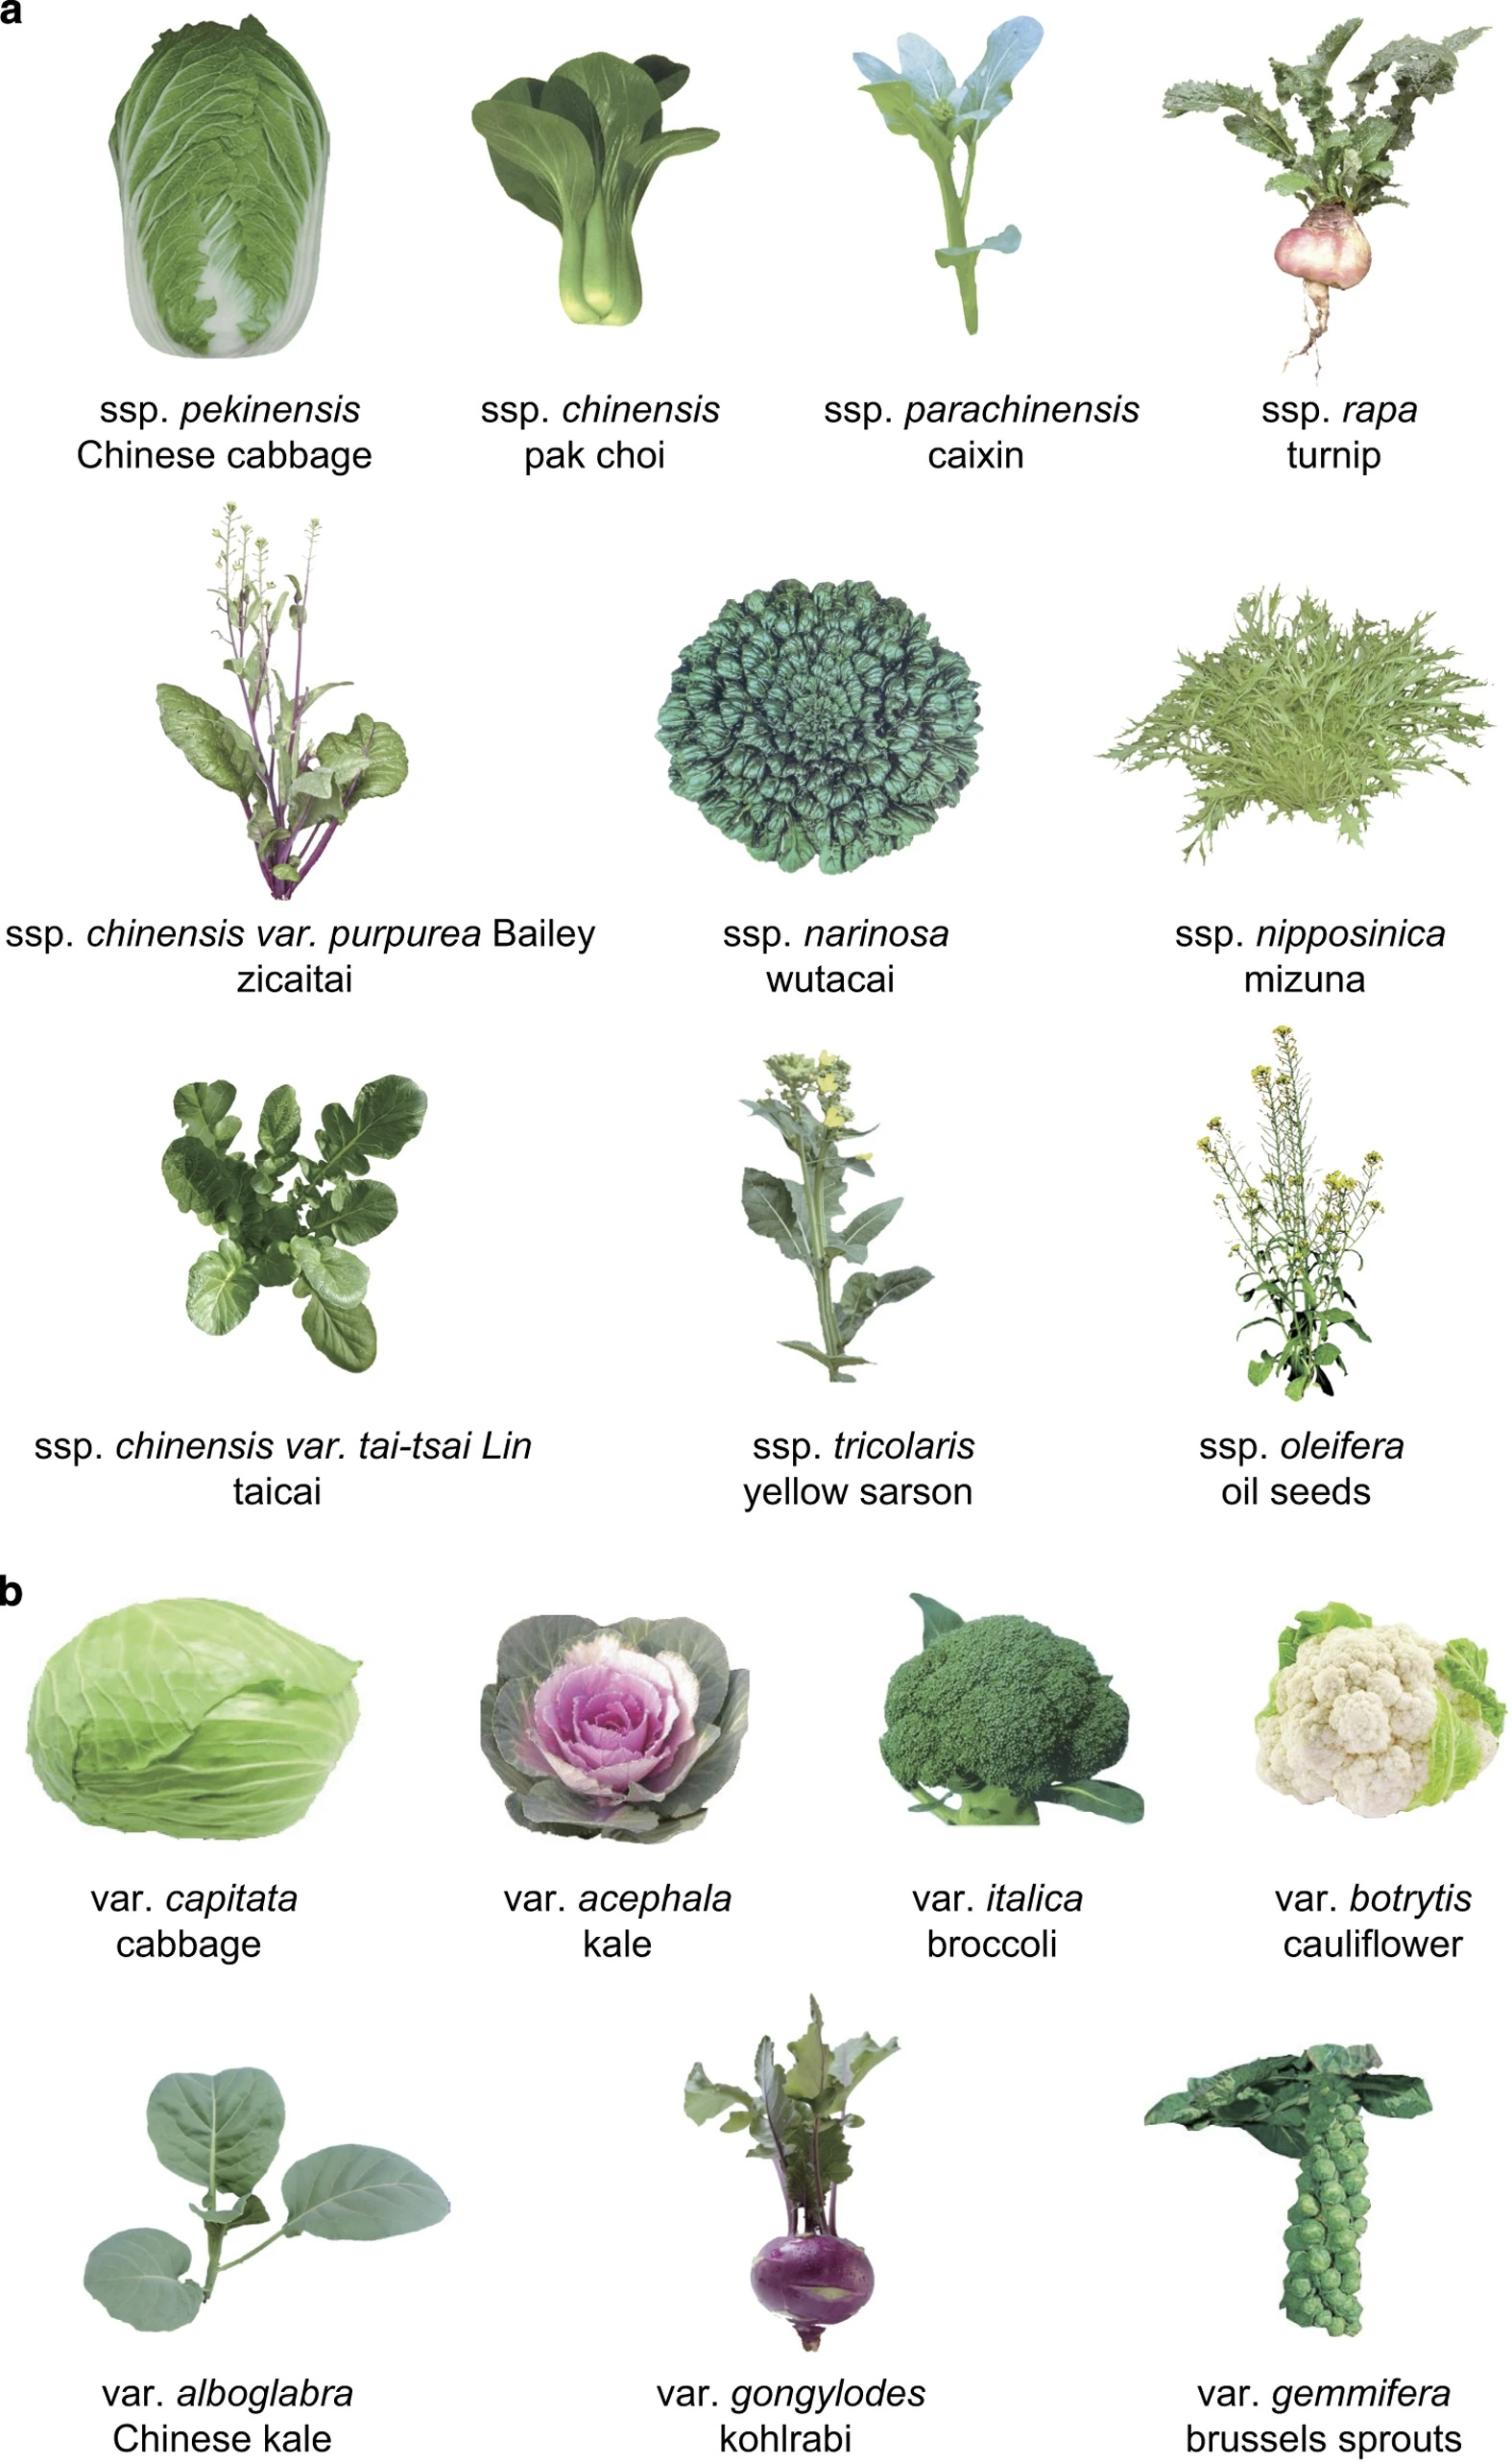
\includegraphics[keepaspectratio, width  = 0.4\textwidth]{img/brassica}
\blfootnote{a) \textit{Brassica rapa} morphotypes; b) \textit{Brassica oleracea} morphotypes - from Cheng \textit{et al }2016}
\end{frame}

\begin{frame}
\begin{columns}
	\begin{column}{0.3\textwidth}	
		Quantitative genetic models work and have been very effective in the last 100 years!
	\end{column}
	\begin{column}{0.7\textwidth}
		\centering
		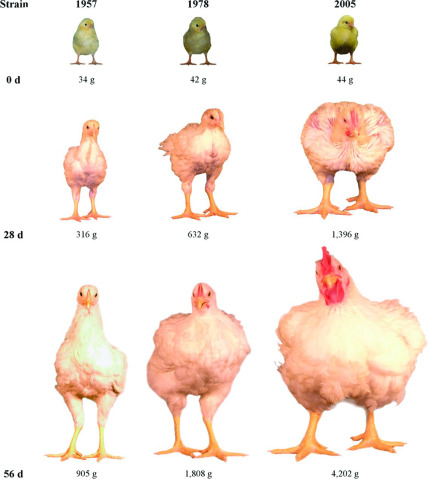
\includegraphics[keepaspectratio, width  =\textwidth]{img/zuidhof_2014} 
	\end{column}
\end{columns}
\blfootnote {Modified from Figure 1 - Zuidhof et al. 2014}
\end{frame}


\begin{frame}
%%%
\begin{columns}
	\begin{column}{0.6\textwidth}
		\centering 	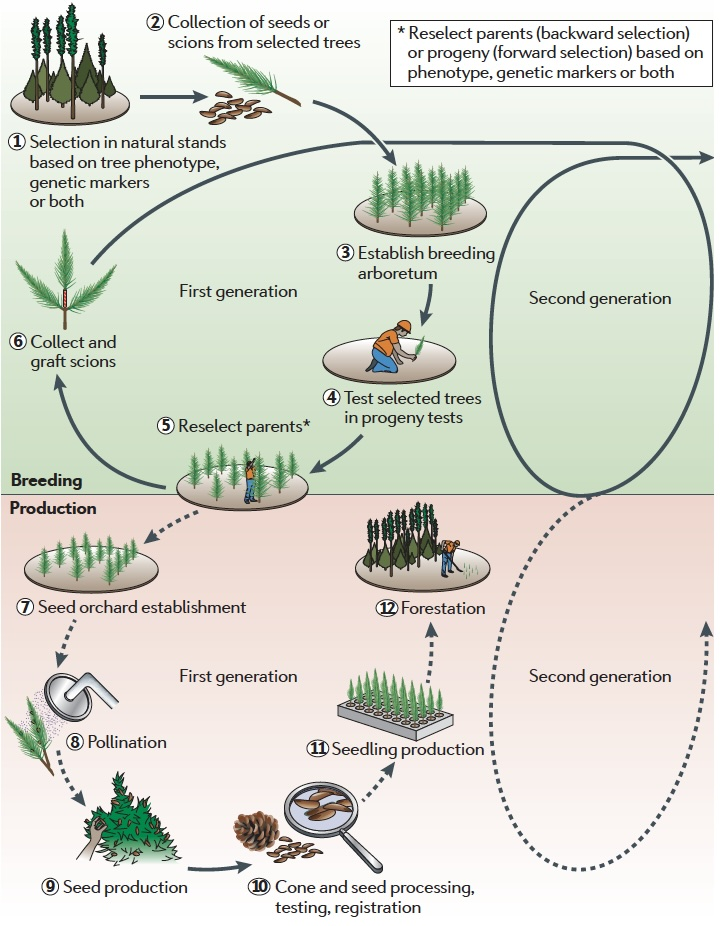
\includegraphics[keepaspectratio, width  = \textwidth]{img/treeImprovement}
	\end{column}
	\begin{column}{0.4\textwidth}
		\textbf{Conventional Tree Breeding\\}
		\pause
		Each cycle takes from 20-30 years!
	\end{column}
\end{columns}
\blfootnote{Image from Neale and Kremer 2011}
\end{frame}

\begin{frame}
\frametitle{Can We Afford to Take That Long?}
\centering
	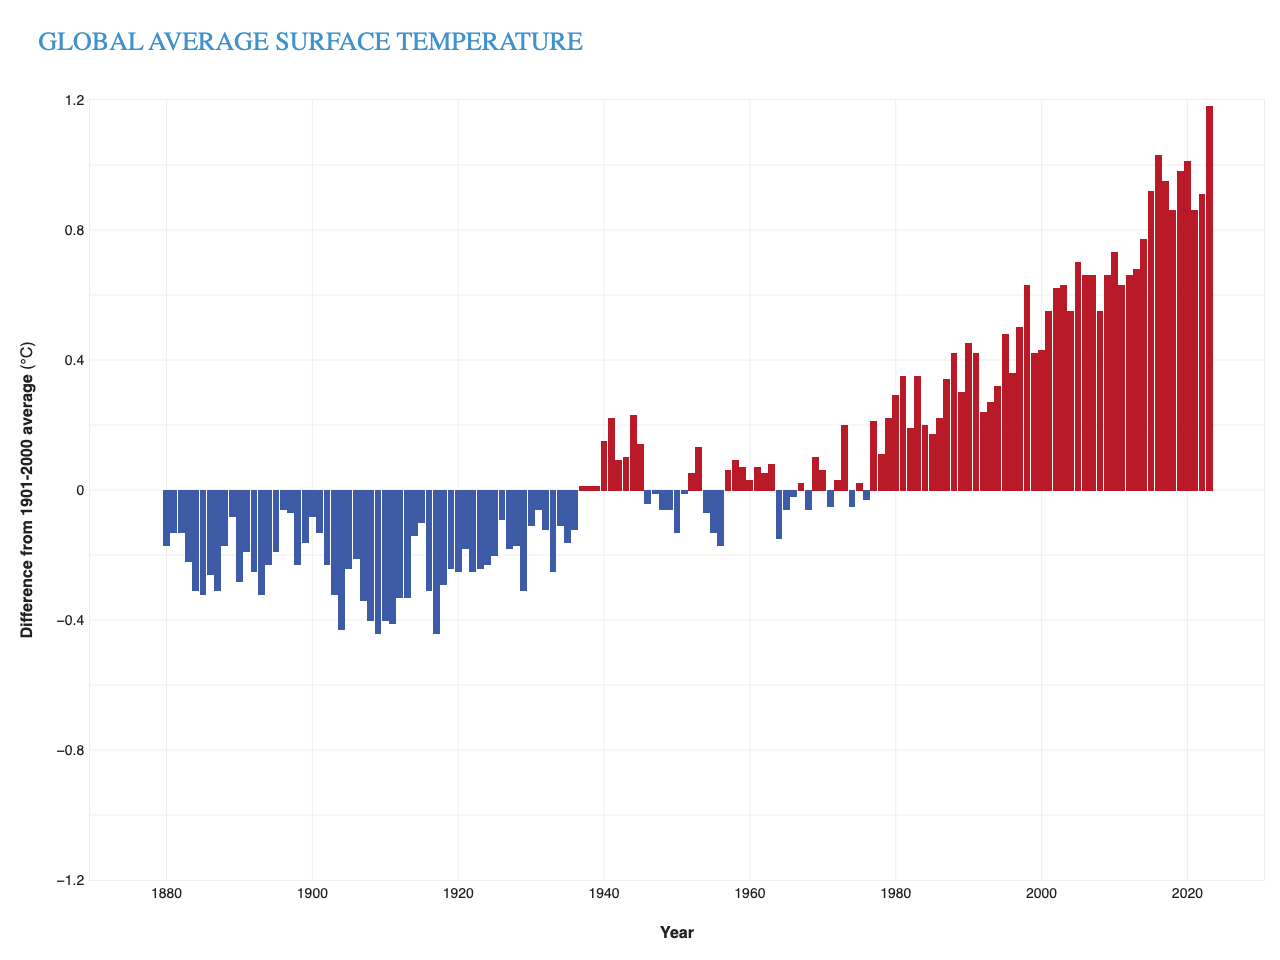
\includegraphics[keepaspectratio, width  = 0.8\textwidth]{img/graph_globalavgsurfacetemp}
	\blfootnote{\url{https://www.climate.gov/news-features/understanding-climate/climate-change-global-temperature} - \textit{Hopefully the webpage still exists...}}
\end{frame}




\begin{frame}
	\Huge How could you advance tree breeding with what you learned in the last three modules?
\end{frame}

\begin{frame}
\Large
	Many of the interventions we may want to take would involve knowing the genes that underly important traits \\
	
	\vspace{20pt}
	For species that are intractable to cultivate in a lab, how can we identify important genetic variation?
\end{frame}



\begin{frame}
\frametitle{Let's Build a Model!}
\centering	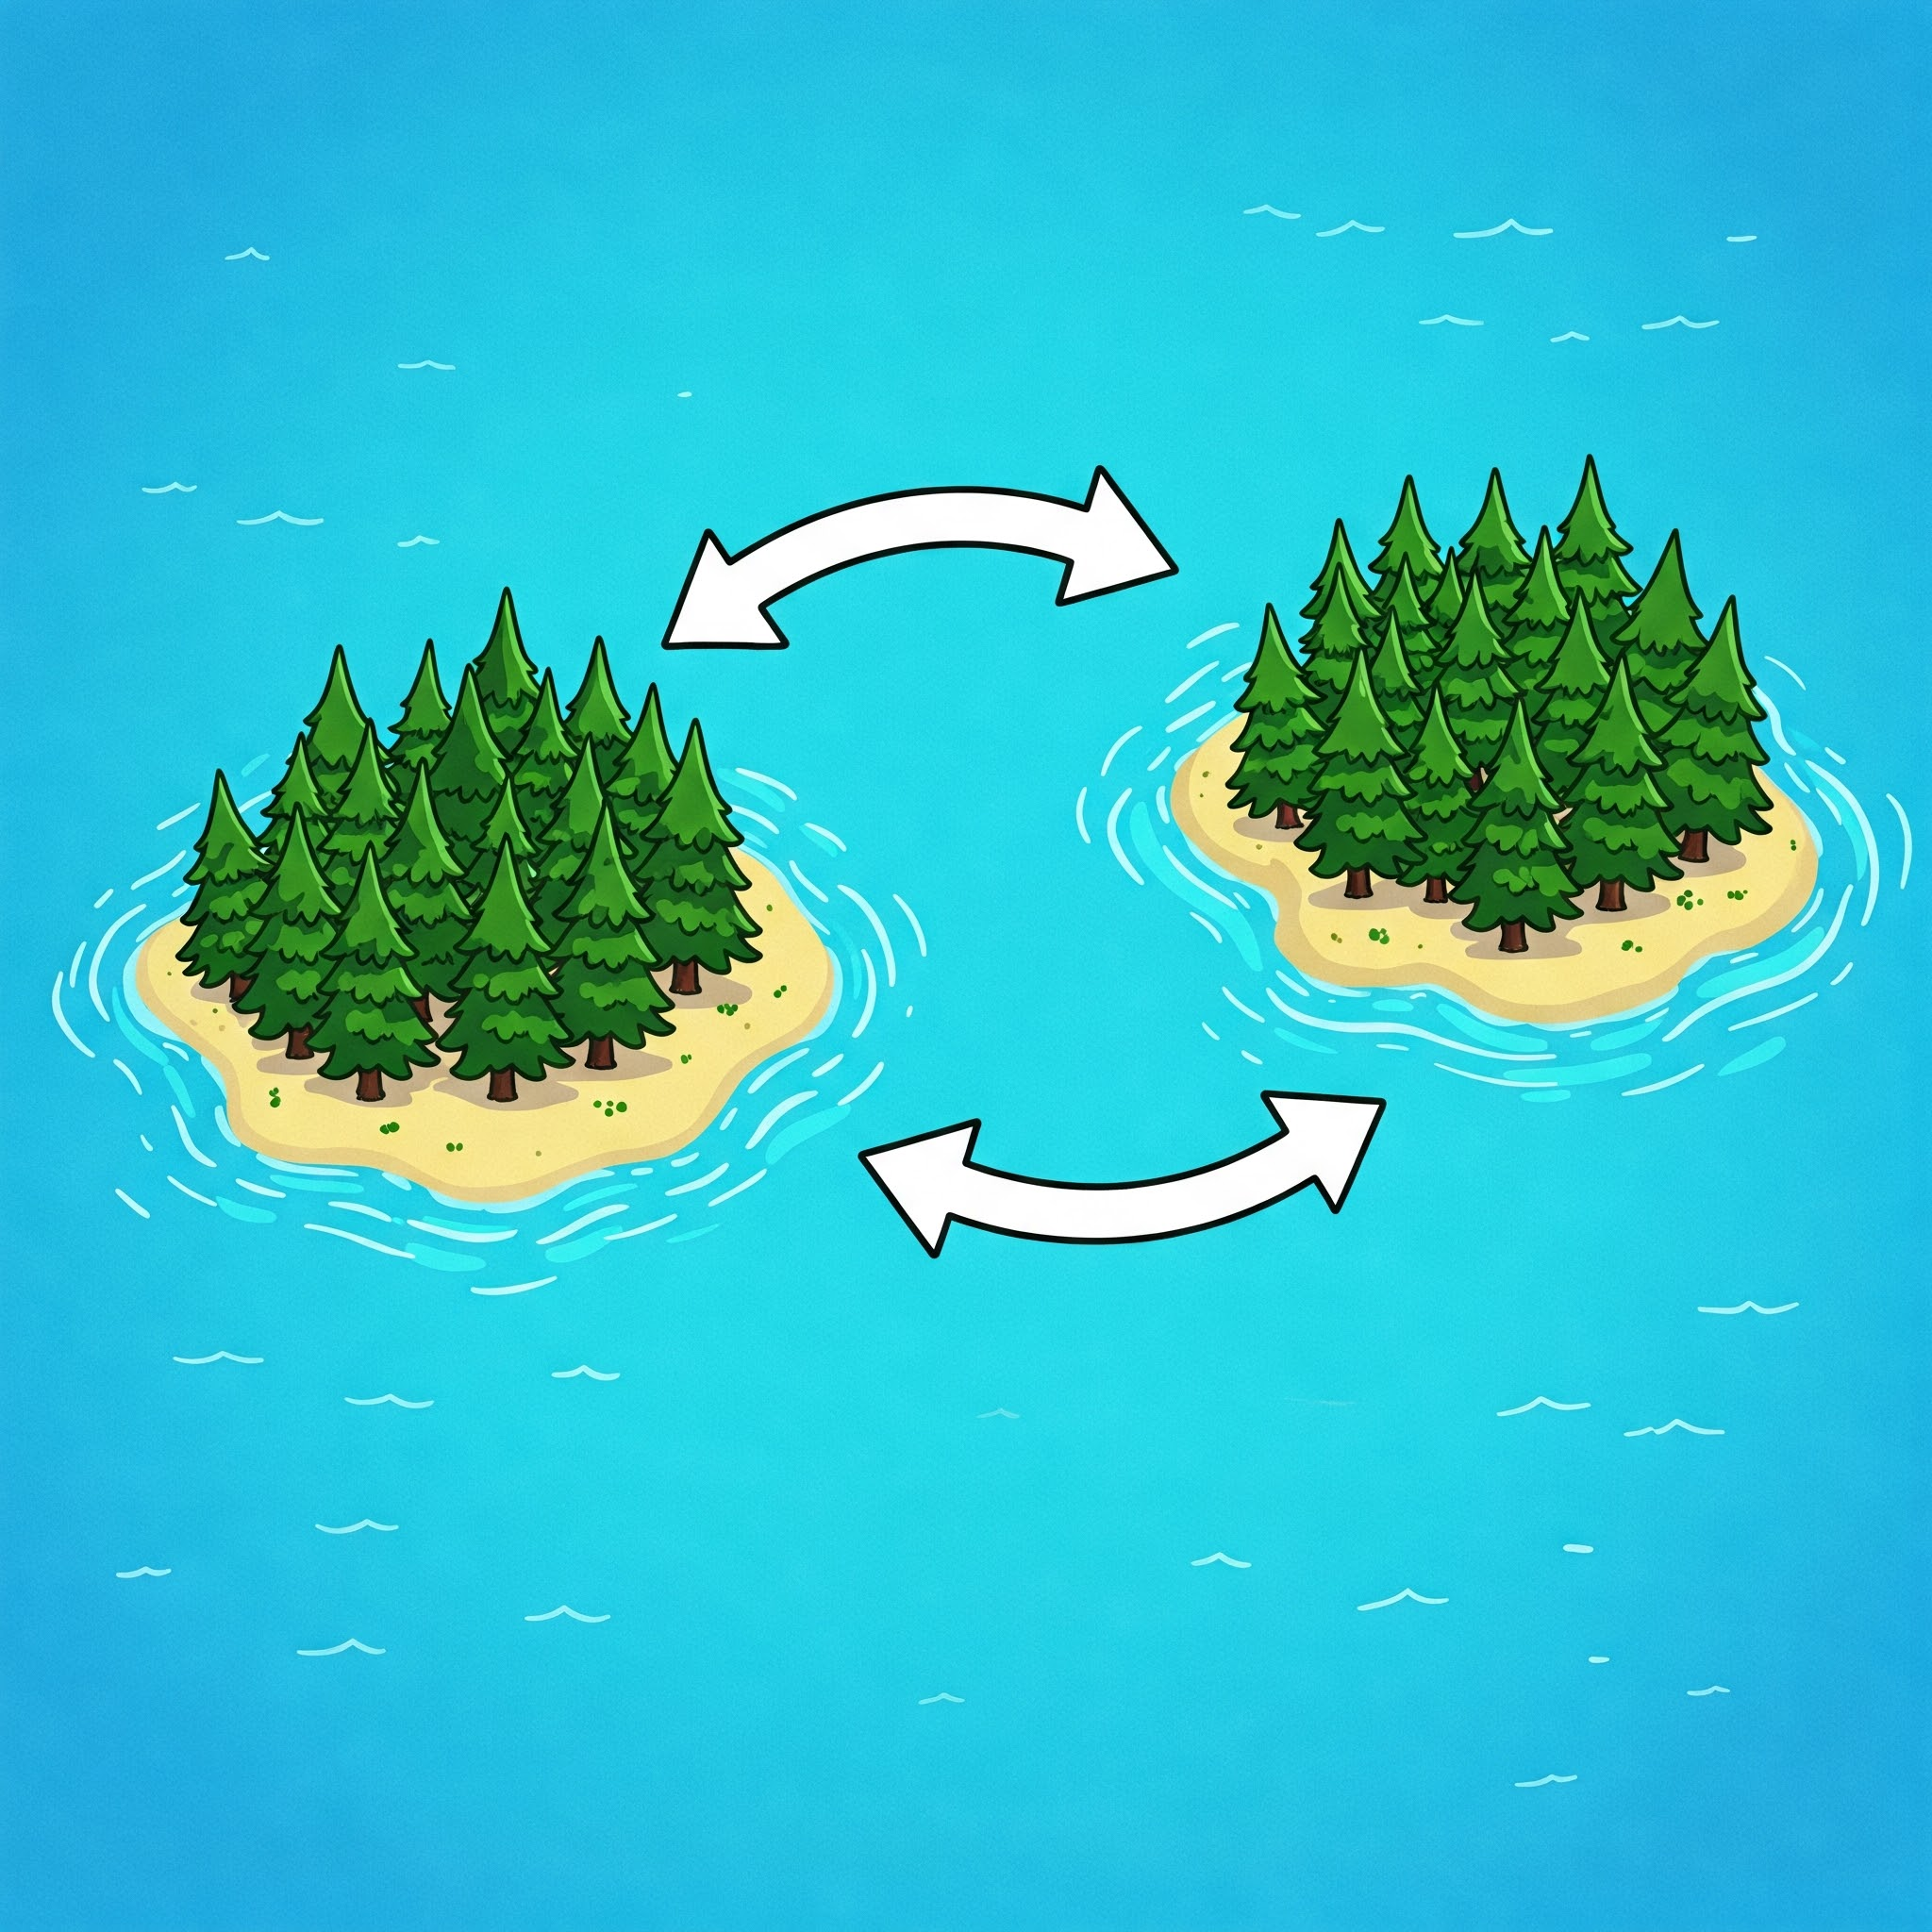
\includegraphics[keepaspectratio, width  = 0.75\textwidth]{img/treeIslands}
\begin{columns}
	\begin{column}{0.4\textwidth}
	\begin{itemize}
	\item[-] Imagine a tree species inhabiting two islands
	\item[-] Pollen flows between them 


\end{itemize}

		\end{column}
	\begin{column}{0.7\textwidth}
		\begin{itemize}
				\item[-] Taller trees are favoured on Island $\#1$
	\item[-] 99.9\% of the time trees pollinate individuals from their own island\footnote{This gives an expected $F_{ST}$ of 0.05}
			\end{itemize}
	\end{column}
\end{columns}
\vspace{15pt}


\end{frame}


\begin{frame}
	\frametitle{	The Genetics of our Model }
	\begin{columns}
		\begin{column}{0.5\textwidth}
			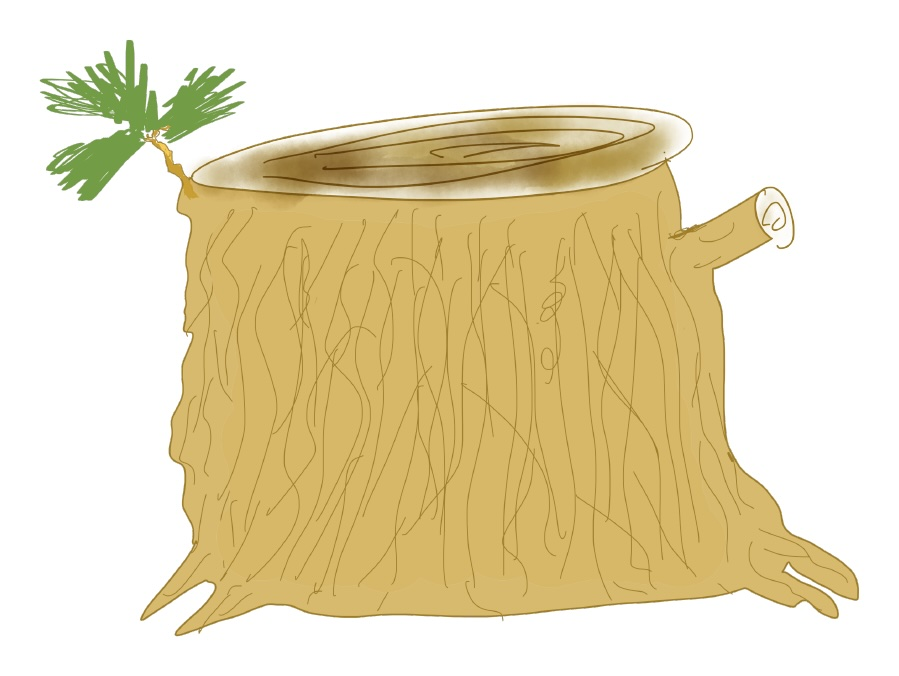
\includegraphics[keepaspectratio, width  = \textwidth]{img/treeStump}
		\end{column}
		\begin{column}{0.6\textwidth}
		\end{column}
	\end{columns}

\end{frame}


\begin{frame}
	\frametitle{	The Genetics of our Model }
	\begin{columns}
		\begin{column}{0.5\textwidth}
			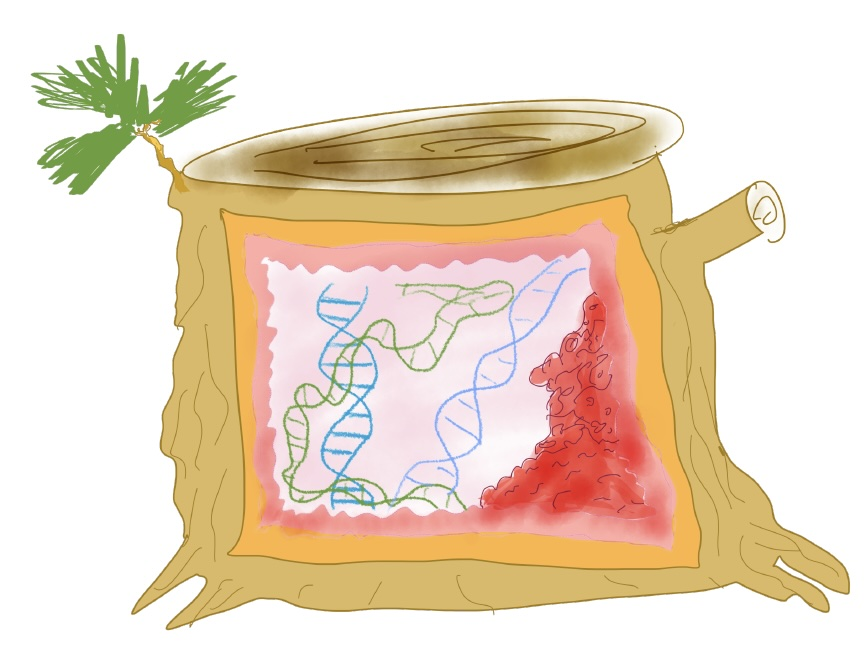
\includegraphics[keepaspectratio, width  = \textwidth]{img/treeGuts}
		\end{column}
		\begin{column}{0.6\textwidth}
			\begin{itemize}
				\item[-] Diploid individuals \pause
				\item[-] The genome is composed of a single chromosome $1cM$ long \pause
				\item[-] Mutations that influence height are co-dominant, with effects drawn from a Gaussian distribution with $\sigma=0.1$ \pause
				\item[-] Mutation rate, $\mu=1\times10^{-9}/bp/generation$ \pause
				\item[-] Heritability of height $h^2=0.4$
			\end{itemize}
		\end{column}
	\end{columns}
\blfootnote{The details on this slide are just for understanding the model. You \textit{will not} be tested on memorizing these numbers and/or parameters}	
\end{frame}



\begin{frame}
	\frametitle{Phenotypic Variation on the Islands}
	\begin{columns}
		\begin{column}{0.65\textwidth}

				\centering
		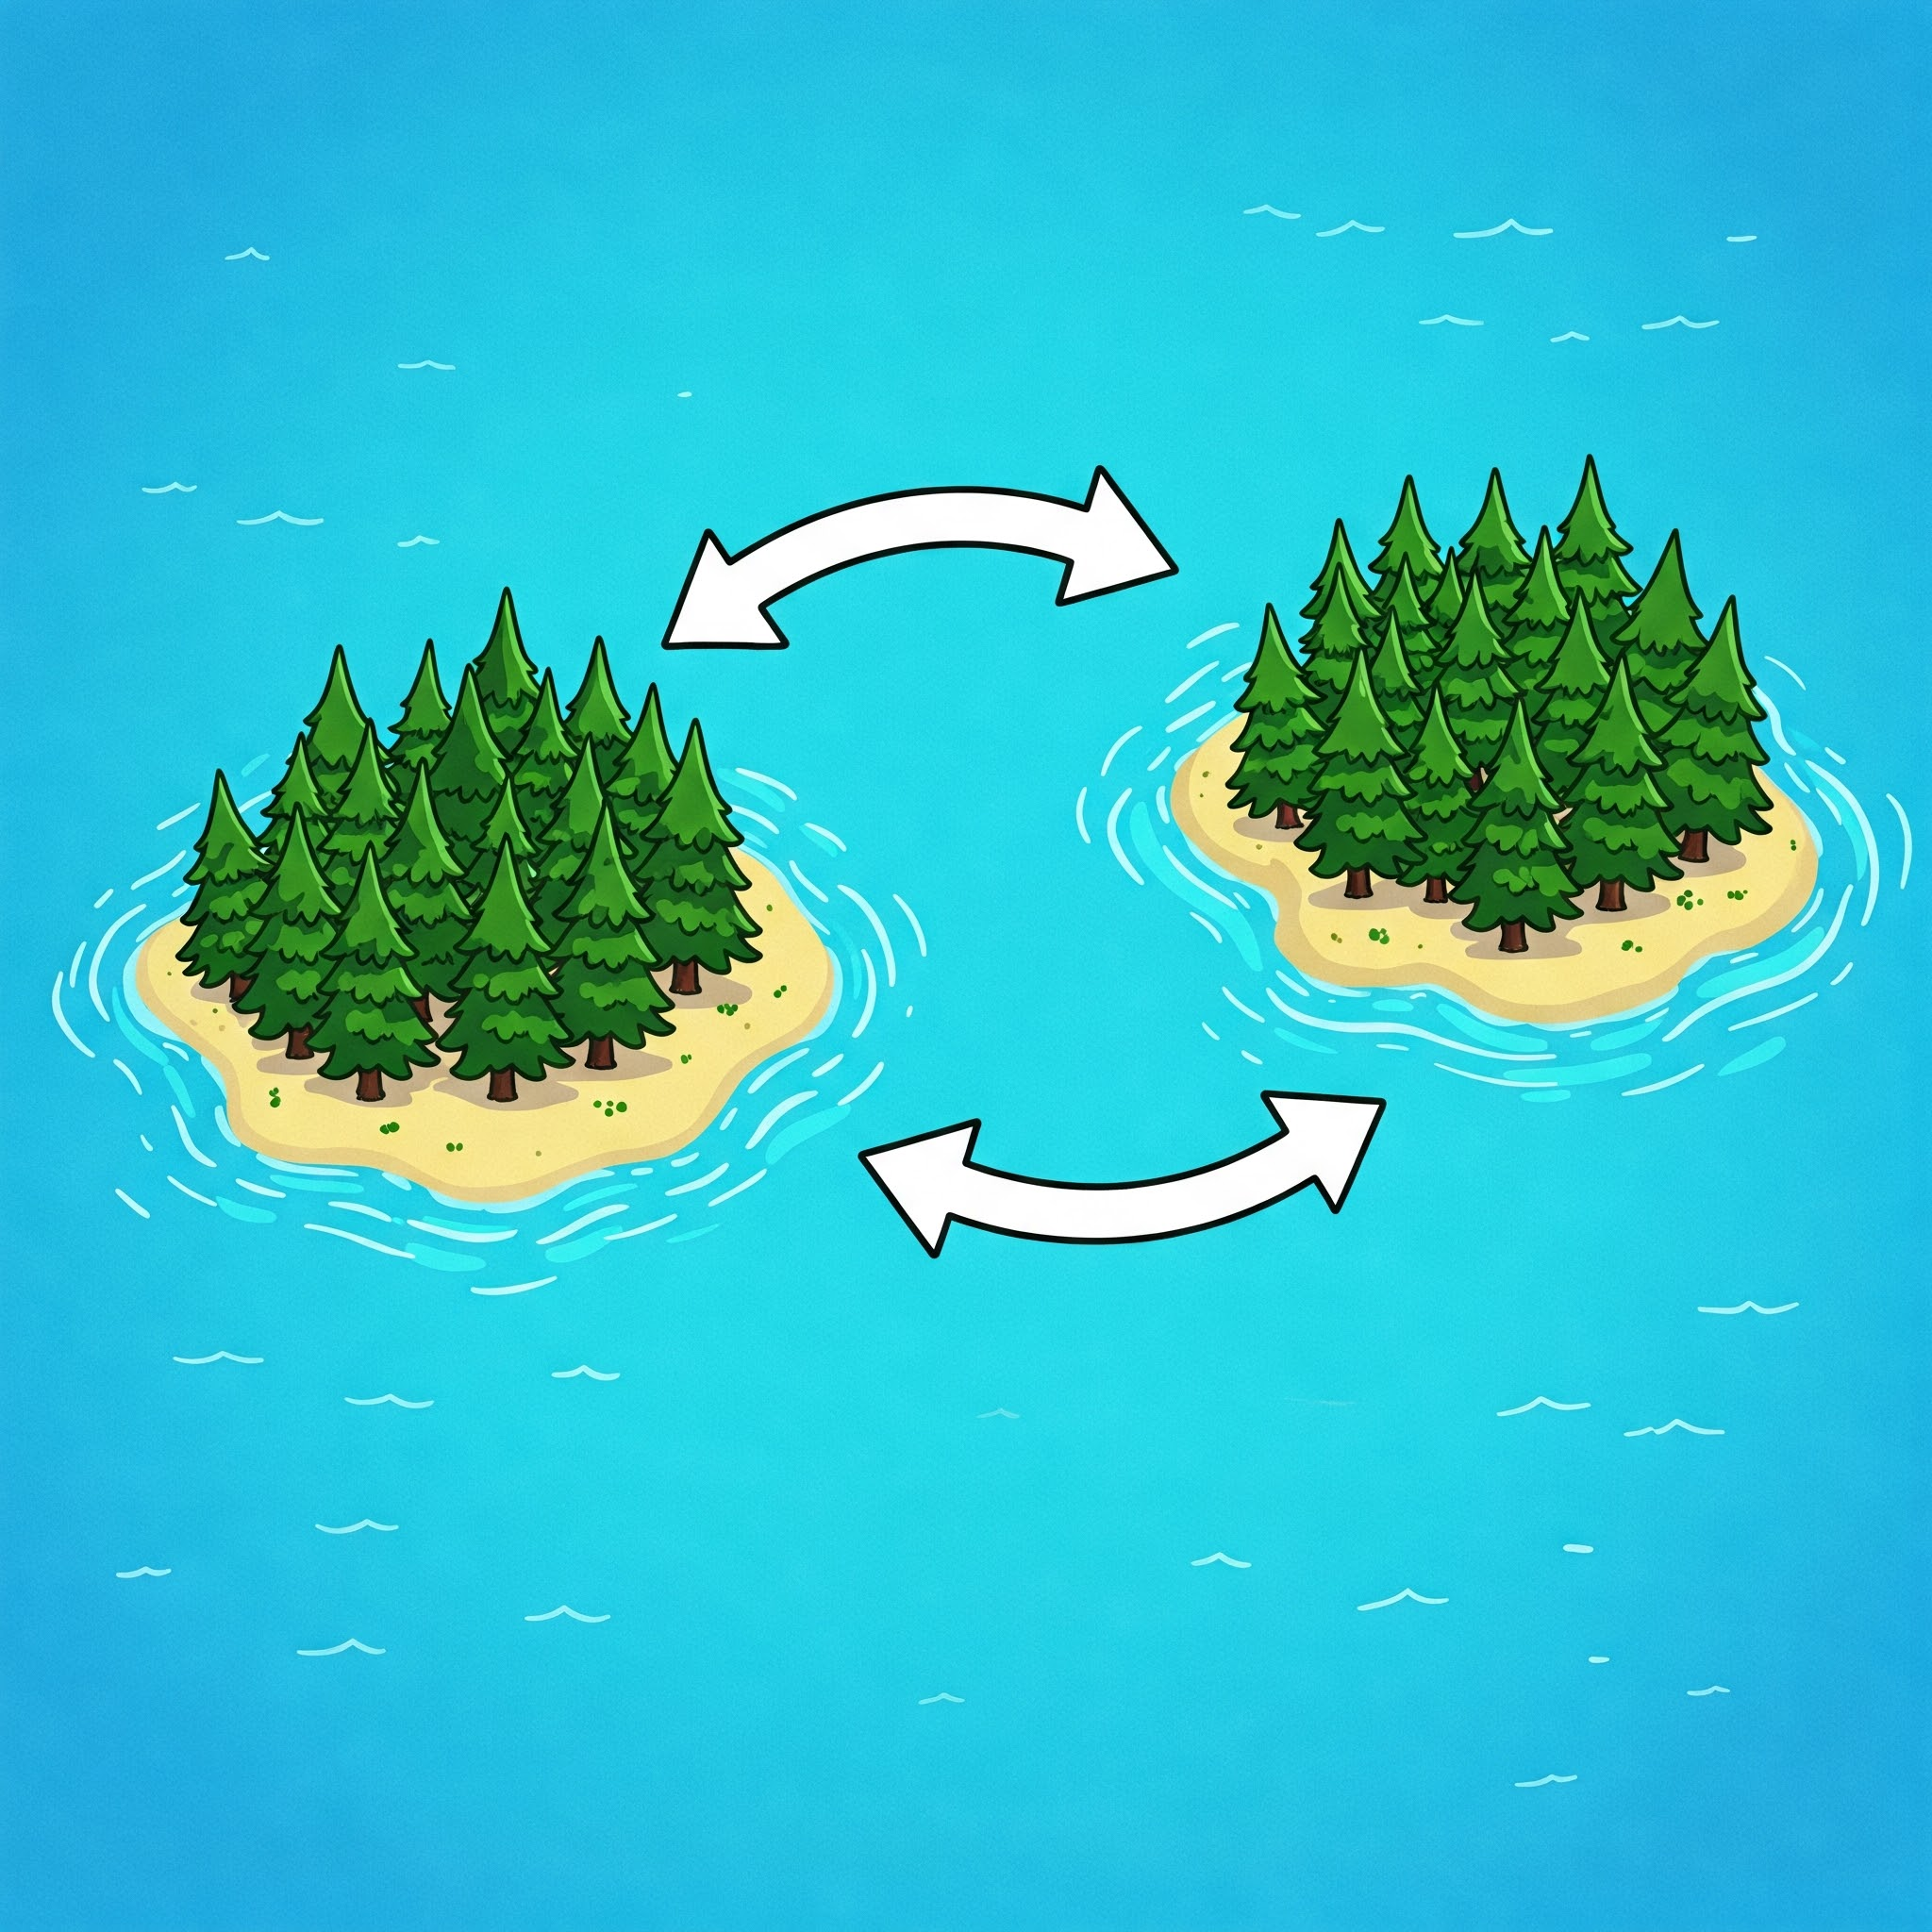
\includegraphics[keepaspectratio, width  = 0.7\textwidth]{img/treeIslands}
						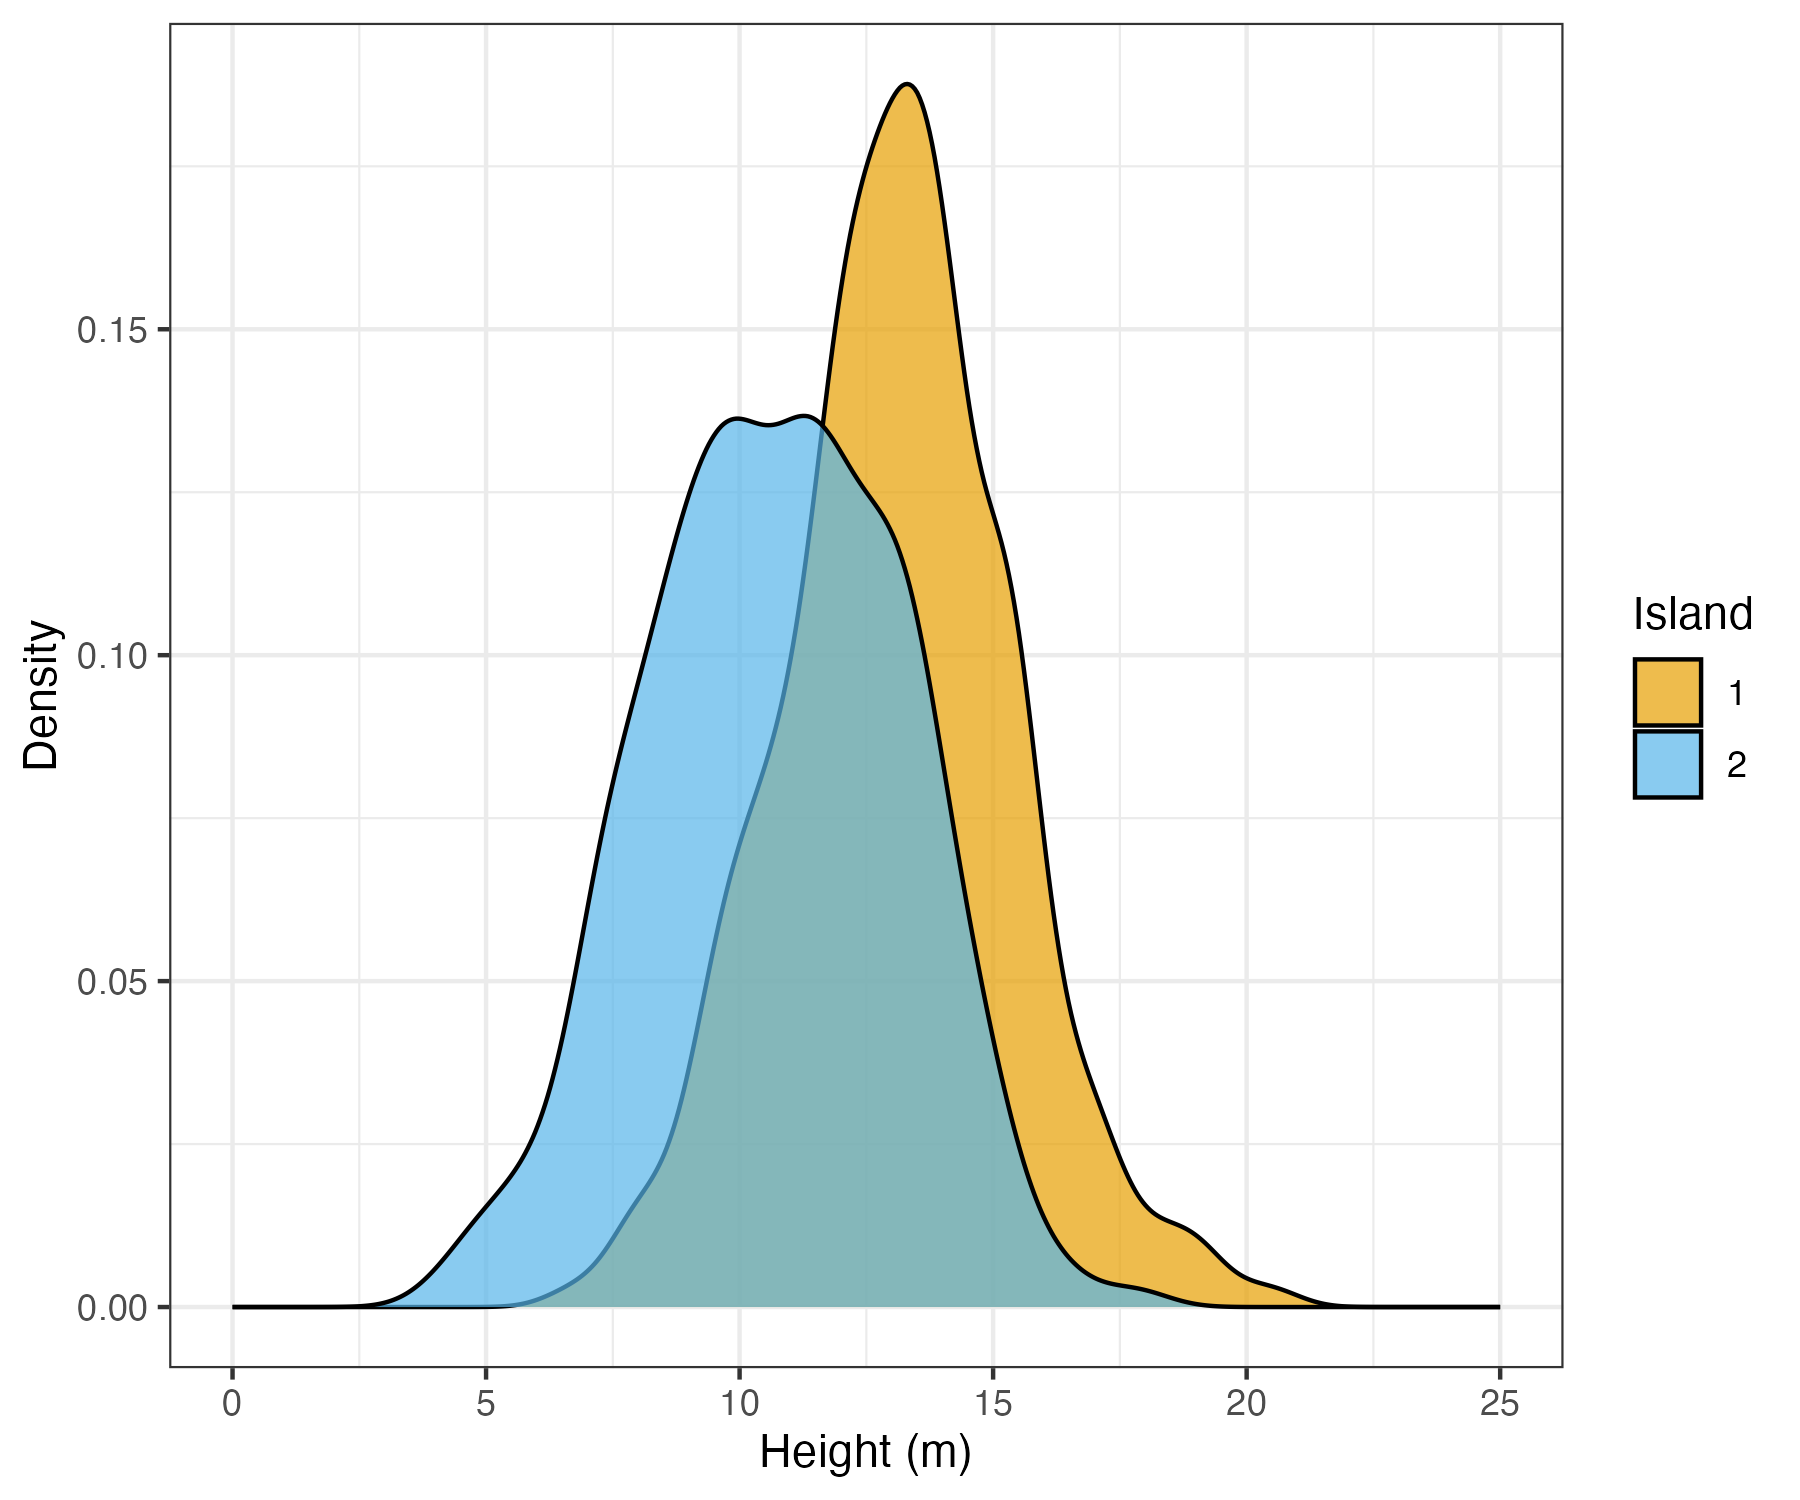
\includegraphics[keepaspectratio, width  = 0.95\textwidth]{img/treePhens.png}				

			
		\end{column}
		\begin{column}{0.4\textwidth}
			\begin{itemize}
				\item[-] Mean height is on 13.11 on Island 1 and 10.71 on Island 2  
				\item[-] This slight difference was statistically significant ($p<<0.001$)
						\end{itemize}
		\end{column}
	\end{columns}
 \end{frame}
 
 
 \begin{frame}
 
 I'll add a picture here of the chromosome with a marker...
 
 \end{frame}
 

\begin{frame}
\frametitle{Testing for Genetic Associations With Tree Height}

To test for an association of a trait (in this case height) with SNP, we can do a statistical regression:

\vspace{15pt}
\Large \centering $\hat{Y}_i \sim \alpha  + \beta_j X_i + \epsilon$ \pause
\vspace{15pt}
\normalsize 
\begin{itemize}

	\item[$\hat{Y}$:] The phenotype of individual $i$
	\item[$\alpha$:] The population mean
	\item[$\beta$:] The effect of marker $j$ on the trait 
	\item[$X_i$:] The number of copies of marker $j$ that individual $i$ possesses
	\item[$\epsilon$:] The effect of the environment on the trait
	
\end{itemize} 

\vspace{15pt}
	
By fitting a regression to the data we can estimate the effect size of a particular marker on a trait and test for statistical significance...

\end{frame}

\begin{frame}
\frametitle{Testing Association at a Single Marker}
	
	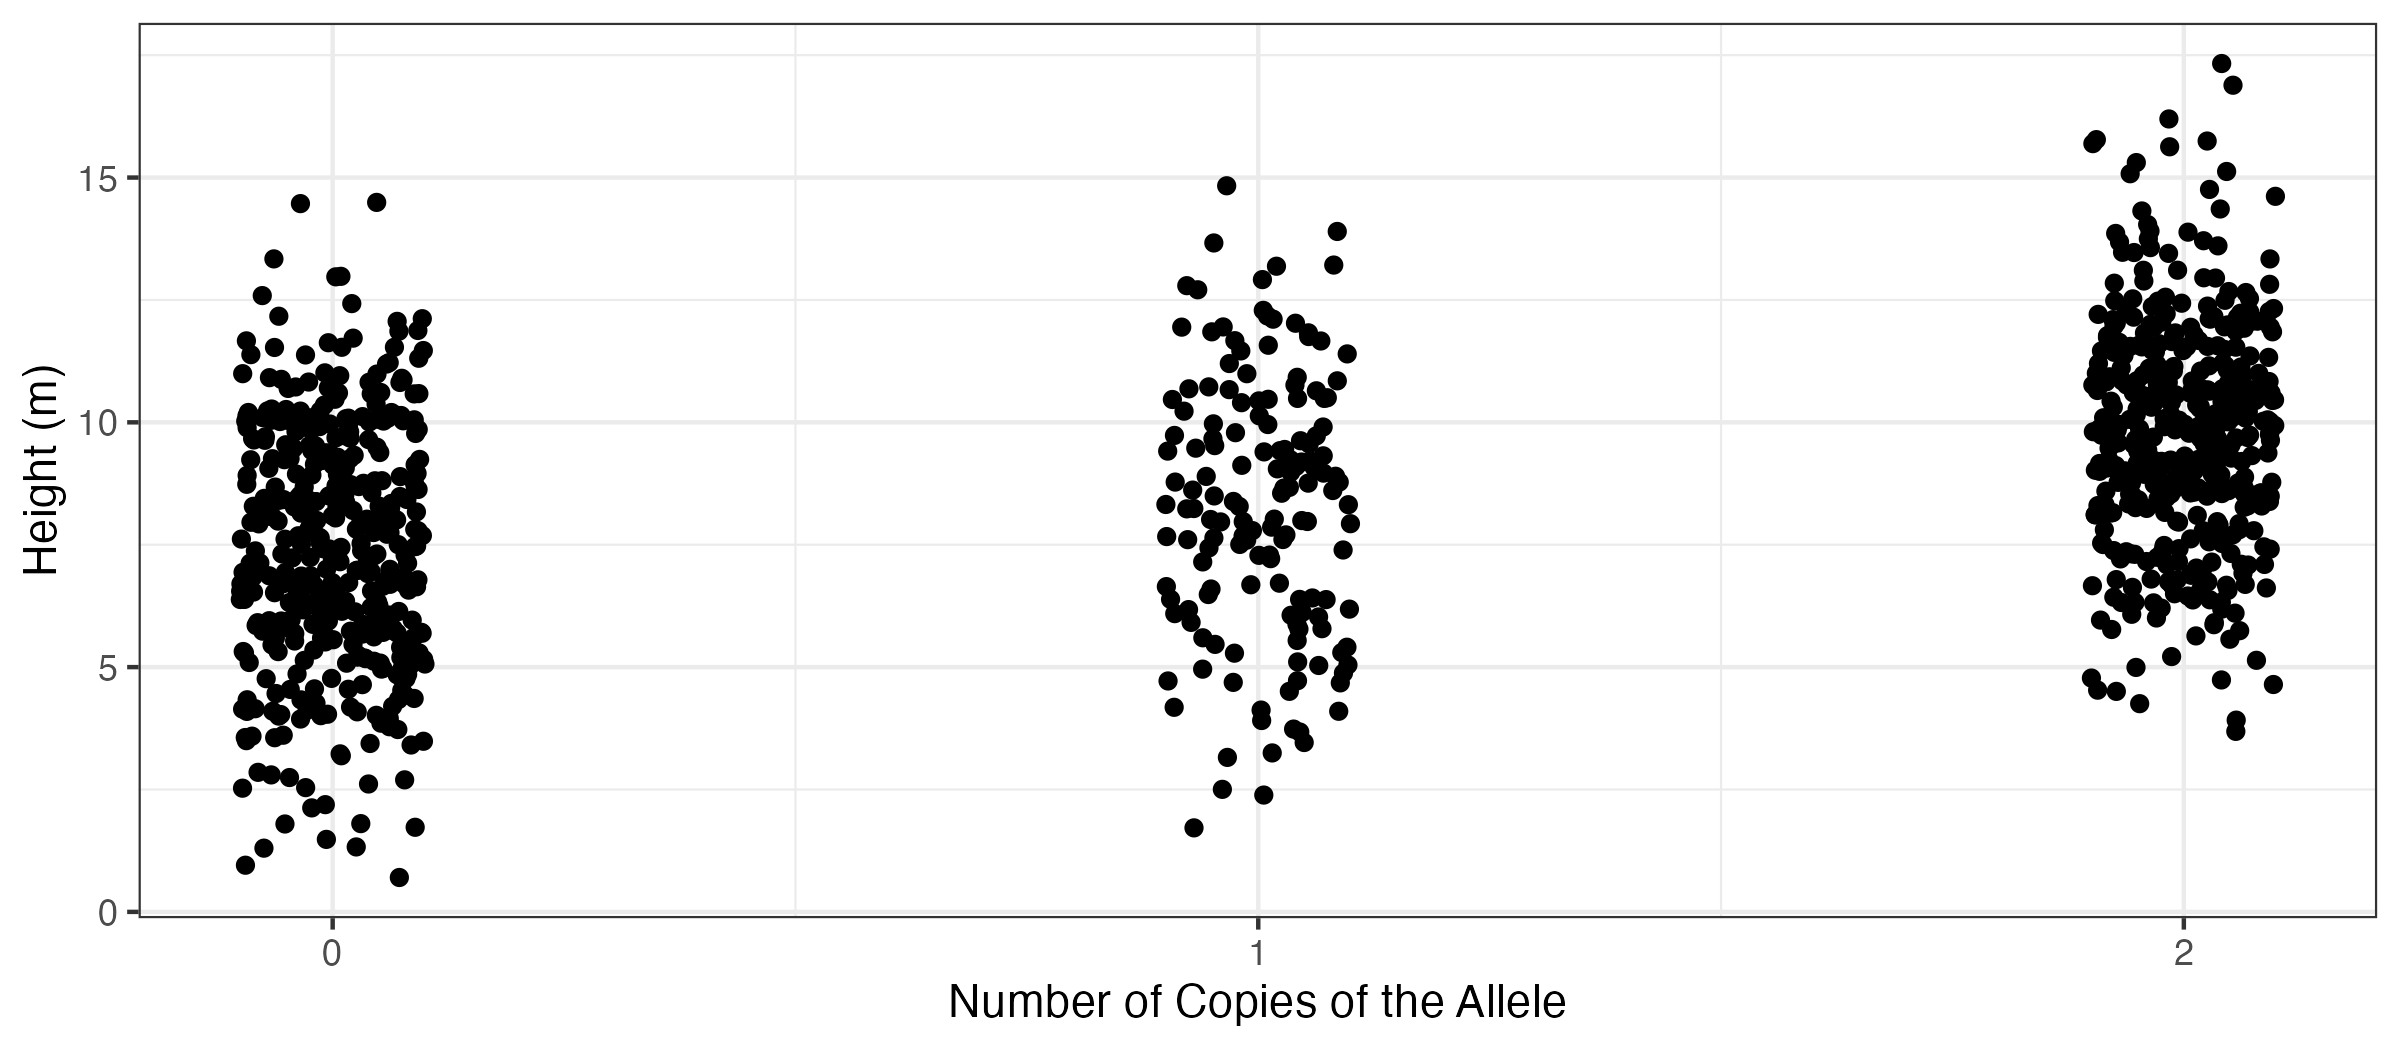
\includegraphics[keepaspectratio, width  = 0.95\textwidth]{img/snp_mod_noLine}				
	
\textit{	The allele is at a frequency of 0.16 across both islands}
\end{frame}


\begin{frame}
	\frametitle{Testing Association at a Single Marker}
	
	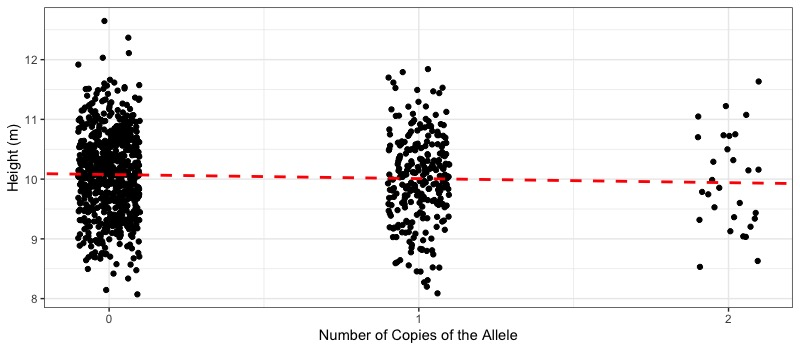
\includegraphics[keepaspectratio, width  = 0.95\textwidth]{img/snp_mod_line}				

\begin{itemize}
	\item[]	The estimated $\beta$ for this SNP is $\beta=-0.07$
	\item[] The $p-value$ for this regression was $p=0.108$
\end{itemize}
\pause 
\vspace{10pt}
\centering \Large What can we say about this marker?


\end{frame}


\begin{frame}
	\frametitle{Genome-Wide Association Study}
	Now, let's look at each SNP across the whole genome \pause
	
		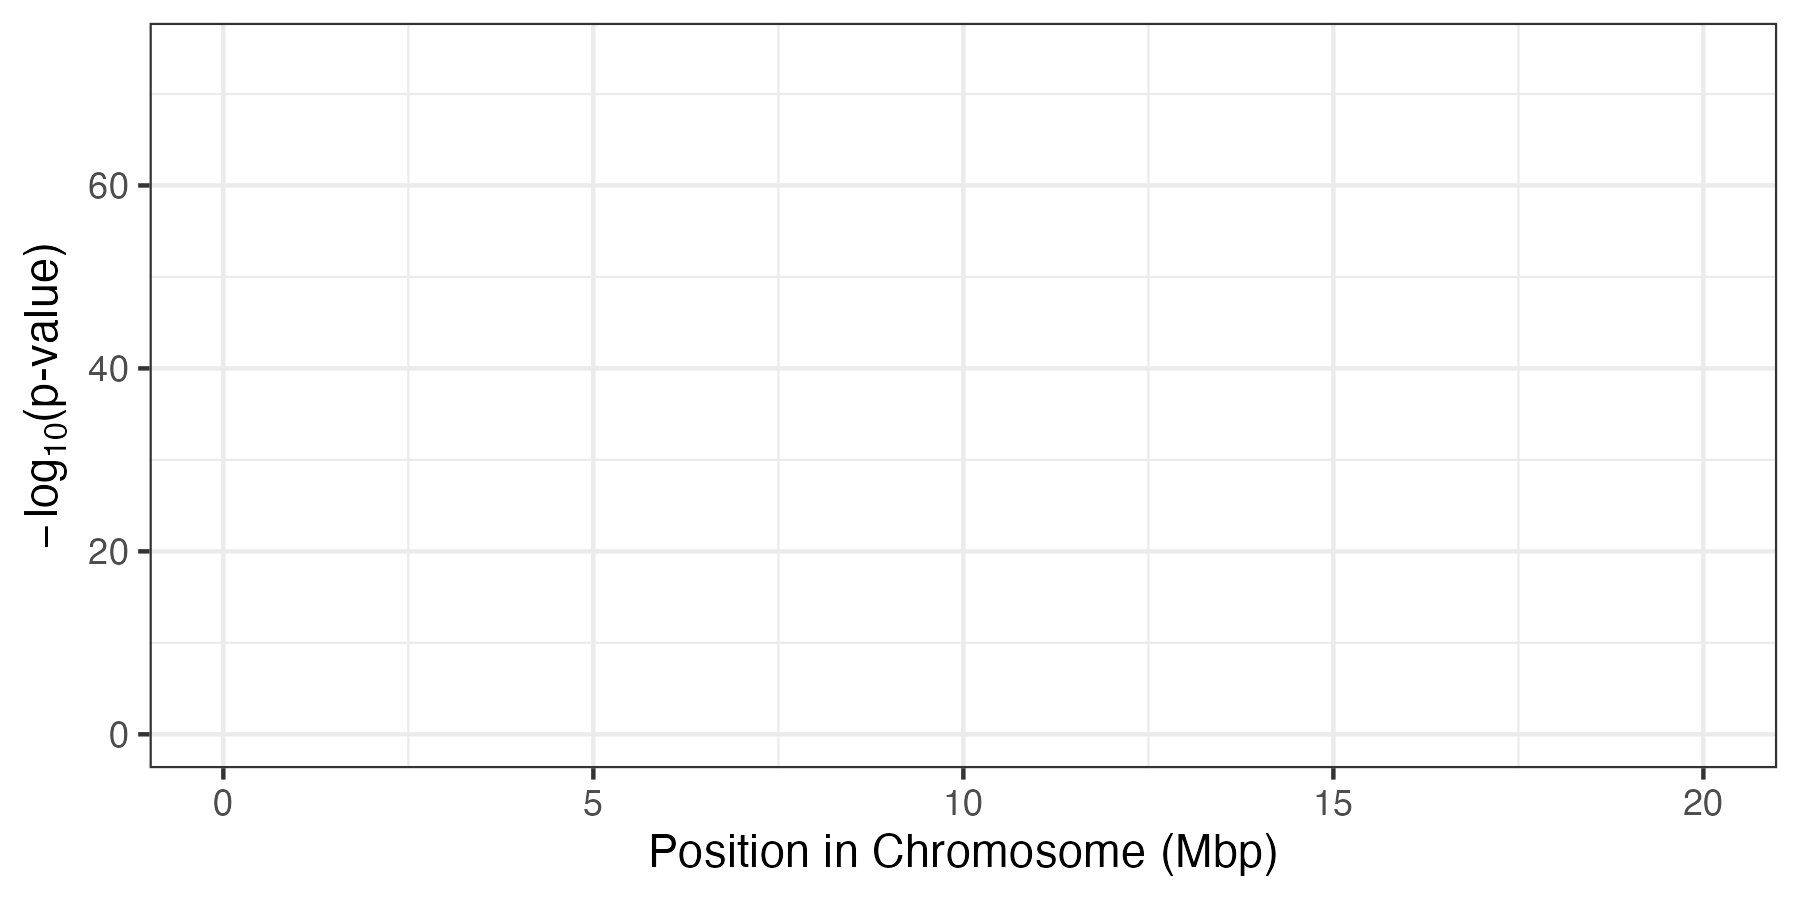
\includegraphics[keepaspectratio, width  = 0.95\textwidth]{img/uncorPlot_noData}				
		
\blfootnote{There's nothing special about $-log_{10}(p-value)$, it's just the $p-value$ of an association expressed in an easy to visualise way}
\end{frame}

\begin{frame}
	\frametitle{Genome-Wide Association Study}
	Now, let's look at each SNP across the whole genome 
	
	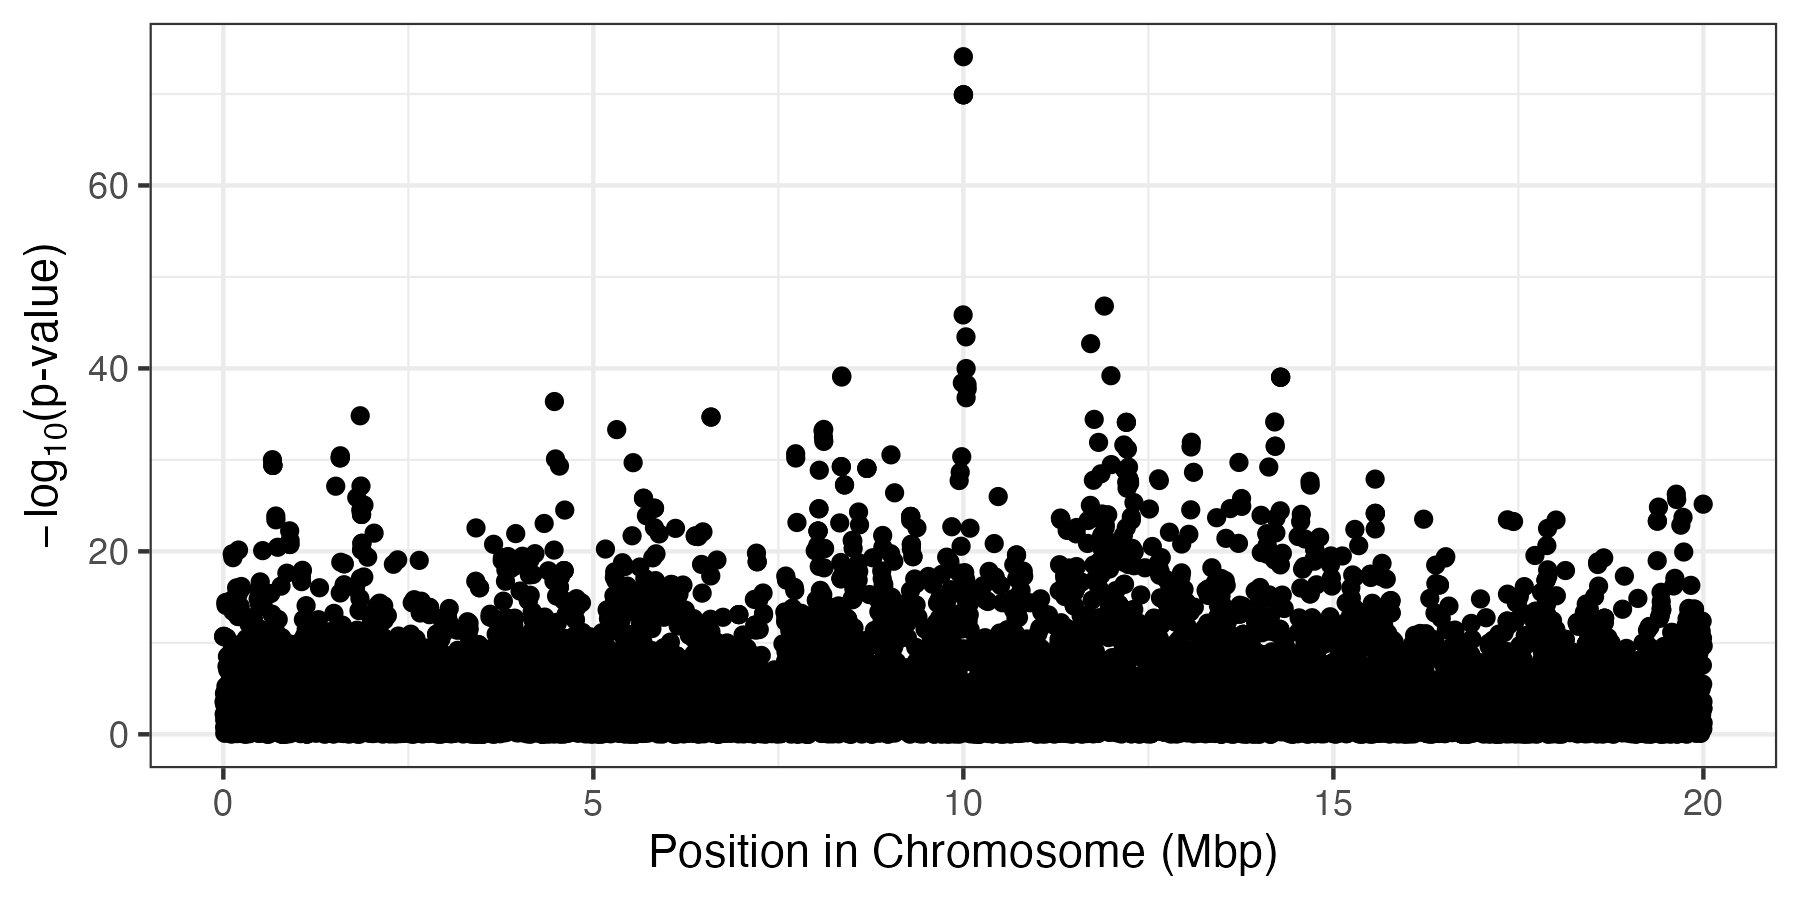
\includegraphics[keepaspectratio, width  = 0.95\textwidth]{img/uncorPlot_Data}				
	
	\blfootnote{There's nothing special about $-log_{10}(p-value)$, it's just the $p-value$ of an association expressed in an easy to visualise way}
\end{frame}


\begin{frame}
	\frametitle{Genome-Wide Association Study}
	Now, let's look at each SNP across the whole genome 
	
	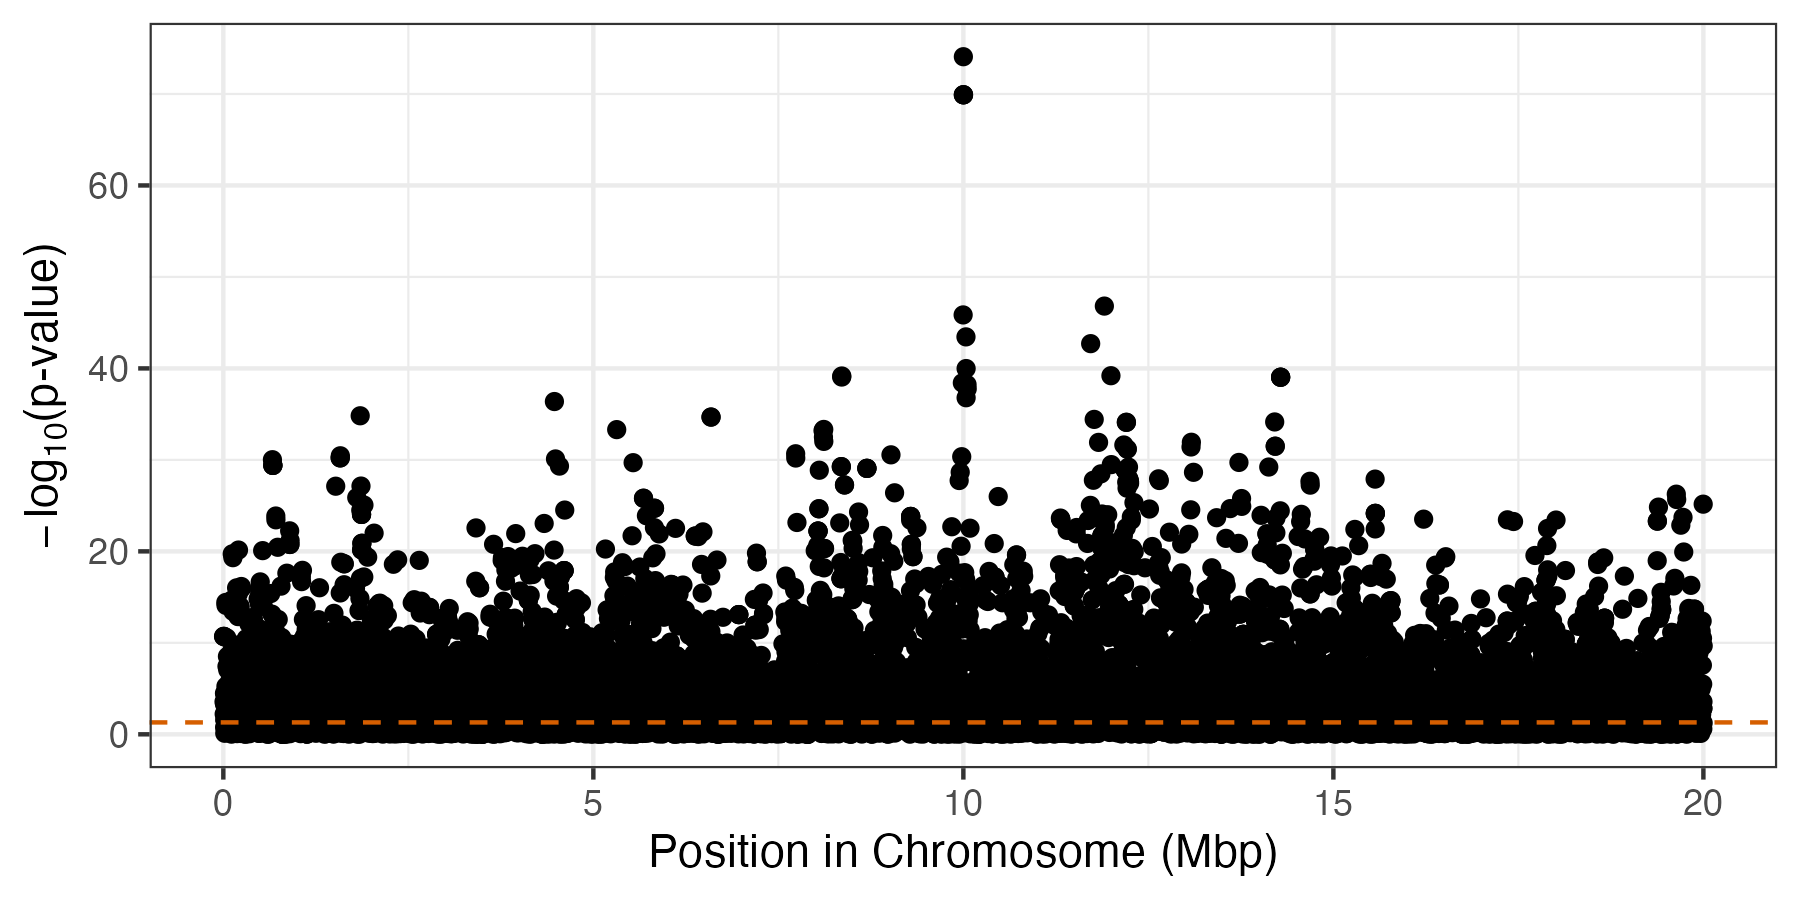
\includegraphics[keepaspectratio, width  = 0.95\textwidth]{img/uncorPlot_DataHline}				
	
	\blfootnote{There's nothing special about $-log_{10}(p-value)$, it's just the $p-value$ of an association expressed in an easy to visualise way}
\end{frame}


\begin{frame}
	\frametitle{Genome-Wide Association Study}
	Now, let's look at each SNP across the whole genome 
	
	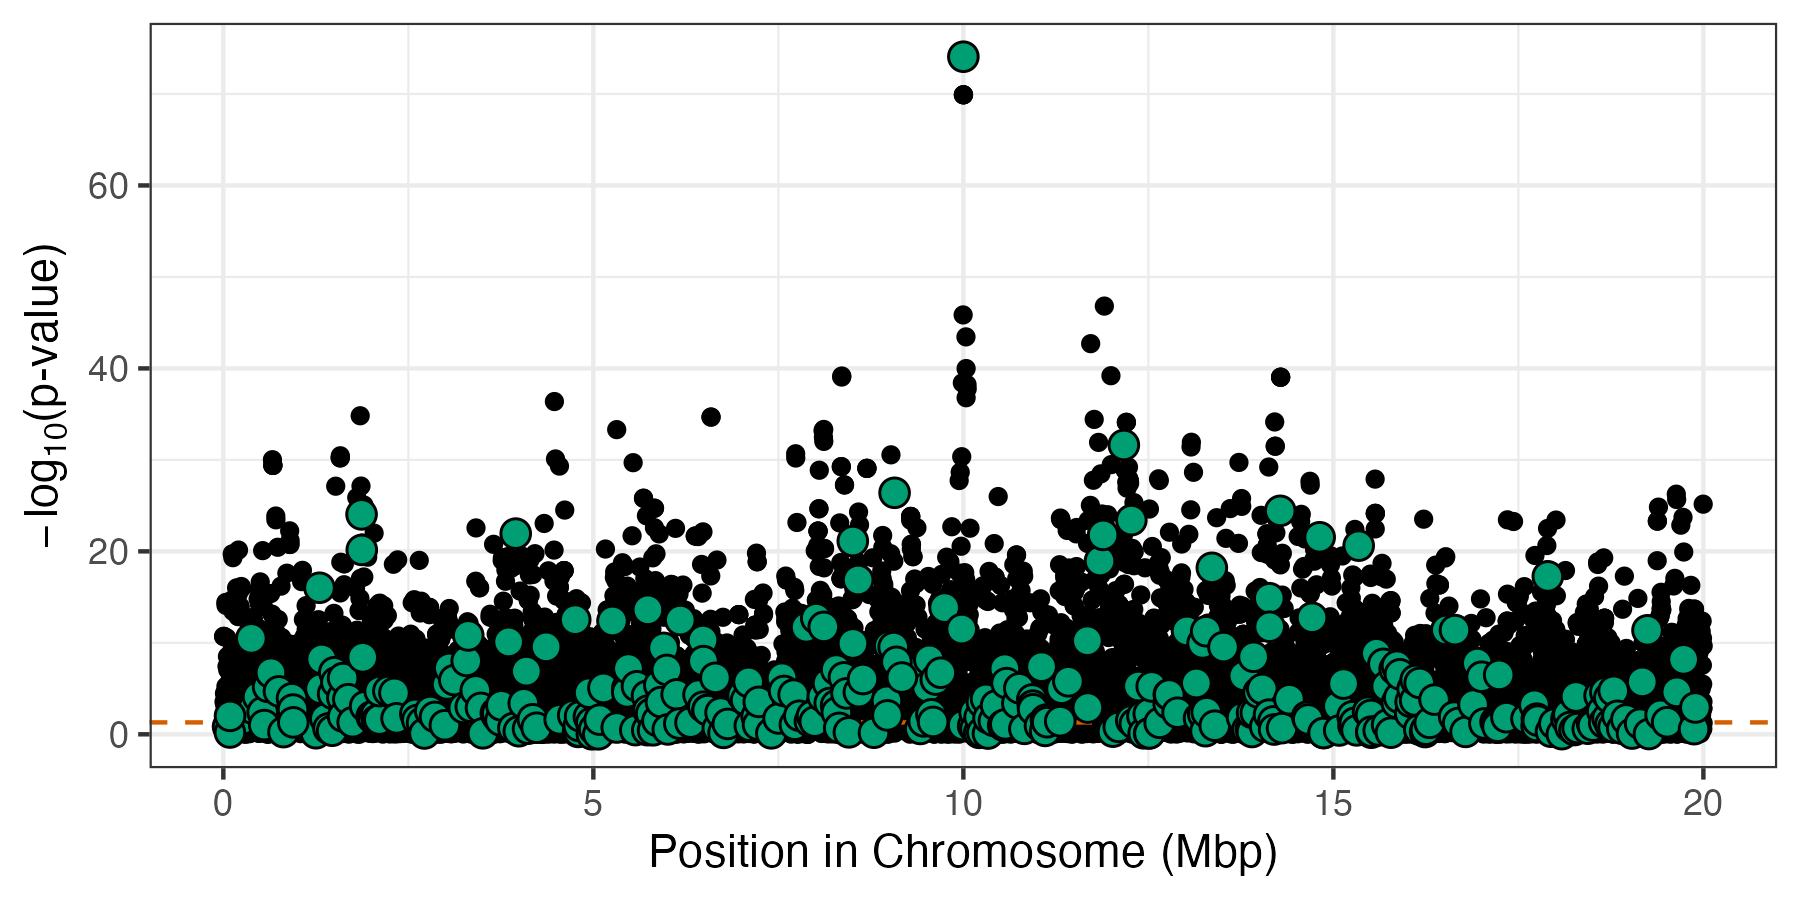
\includegraphics[keepaspectratio, width  = 0.95\textwidth]{img/uncorPlot_DataHlineTrue}				
	
	\blfootnote{There's nothing special about $-log_{10}(p-value)$, it's just the $p-value$ of an association expressed in an easy to visualise way}
\end{frame}


\begin{frame}
	\Huge
	Can anyone think of any problems with the approach we have taken so far?

\end{frame}

\begin{frame}
	
	\frametitle{Association Genetics Caveat: Population Structure/Relatedness}


%%%
\begin{columns}
	\begin{column}{0.4\textwidth}
		
\includegraphics[keepaspectratio, width  = \textwidth]{img/alan}				
	\end{column}
	\begin{column}{0.7\textwidth}
		\begin{itemize}
			\item British people \textit{really} like tea \\
			\vspace{15pt}
			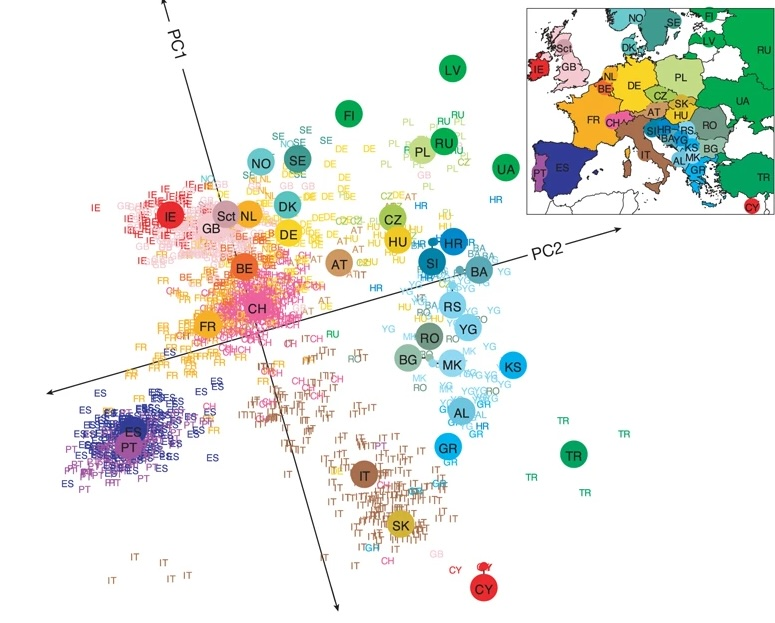
\includegraphics[keepaspectratio, width  = 0.9\textwidth]{img/human_pca}				
		\end{itemize}
	\end{column}
\end{columns}
\blfootnote{Figure modified from: Novembre et al 2008 - \textit{Nature}}
\end{frame}


\begin{frame}
	
	\frametitle{Association Genetics Caveat: Population Structure/Relatedness}

\begin{columns}
	\begin{column}{0.4\textwidth}
		
\includegraphics[keepaspectratio, width  = \textwidth]{img/alan}				
	\end{column}
	\begin{column}{0.7\textwidth}
		\begin{itemize}
			\item British people \textit{really} like tea 
			\vspace{7.5pt}
			\item Genetic drift has led to slight differences in allele frequencies in the UK compared to other places
			\vspace{7.5pt}
			\item Could lead to genetic associations for tea preference
			\vspace{7.5pt}
			\item\textbf{ A relatedness structure among sampled individuals can lead to spurious genetic associations}
			
			\vspace{10pt}
		\end{itemize}
	\end{column}
\end{columns}
\blfootnote{ Tea drinking in the UK has a clear cultural basis}
\end{frame}


\begin{frame}
	
	\frametitle{Association Genetics Caveat: Population Structure/Relatedness}
	
		\begin{columns}
		\begin{column}{0.65\textwidth}
			
			\centering
			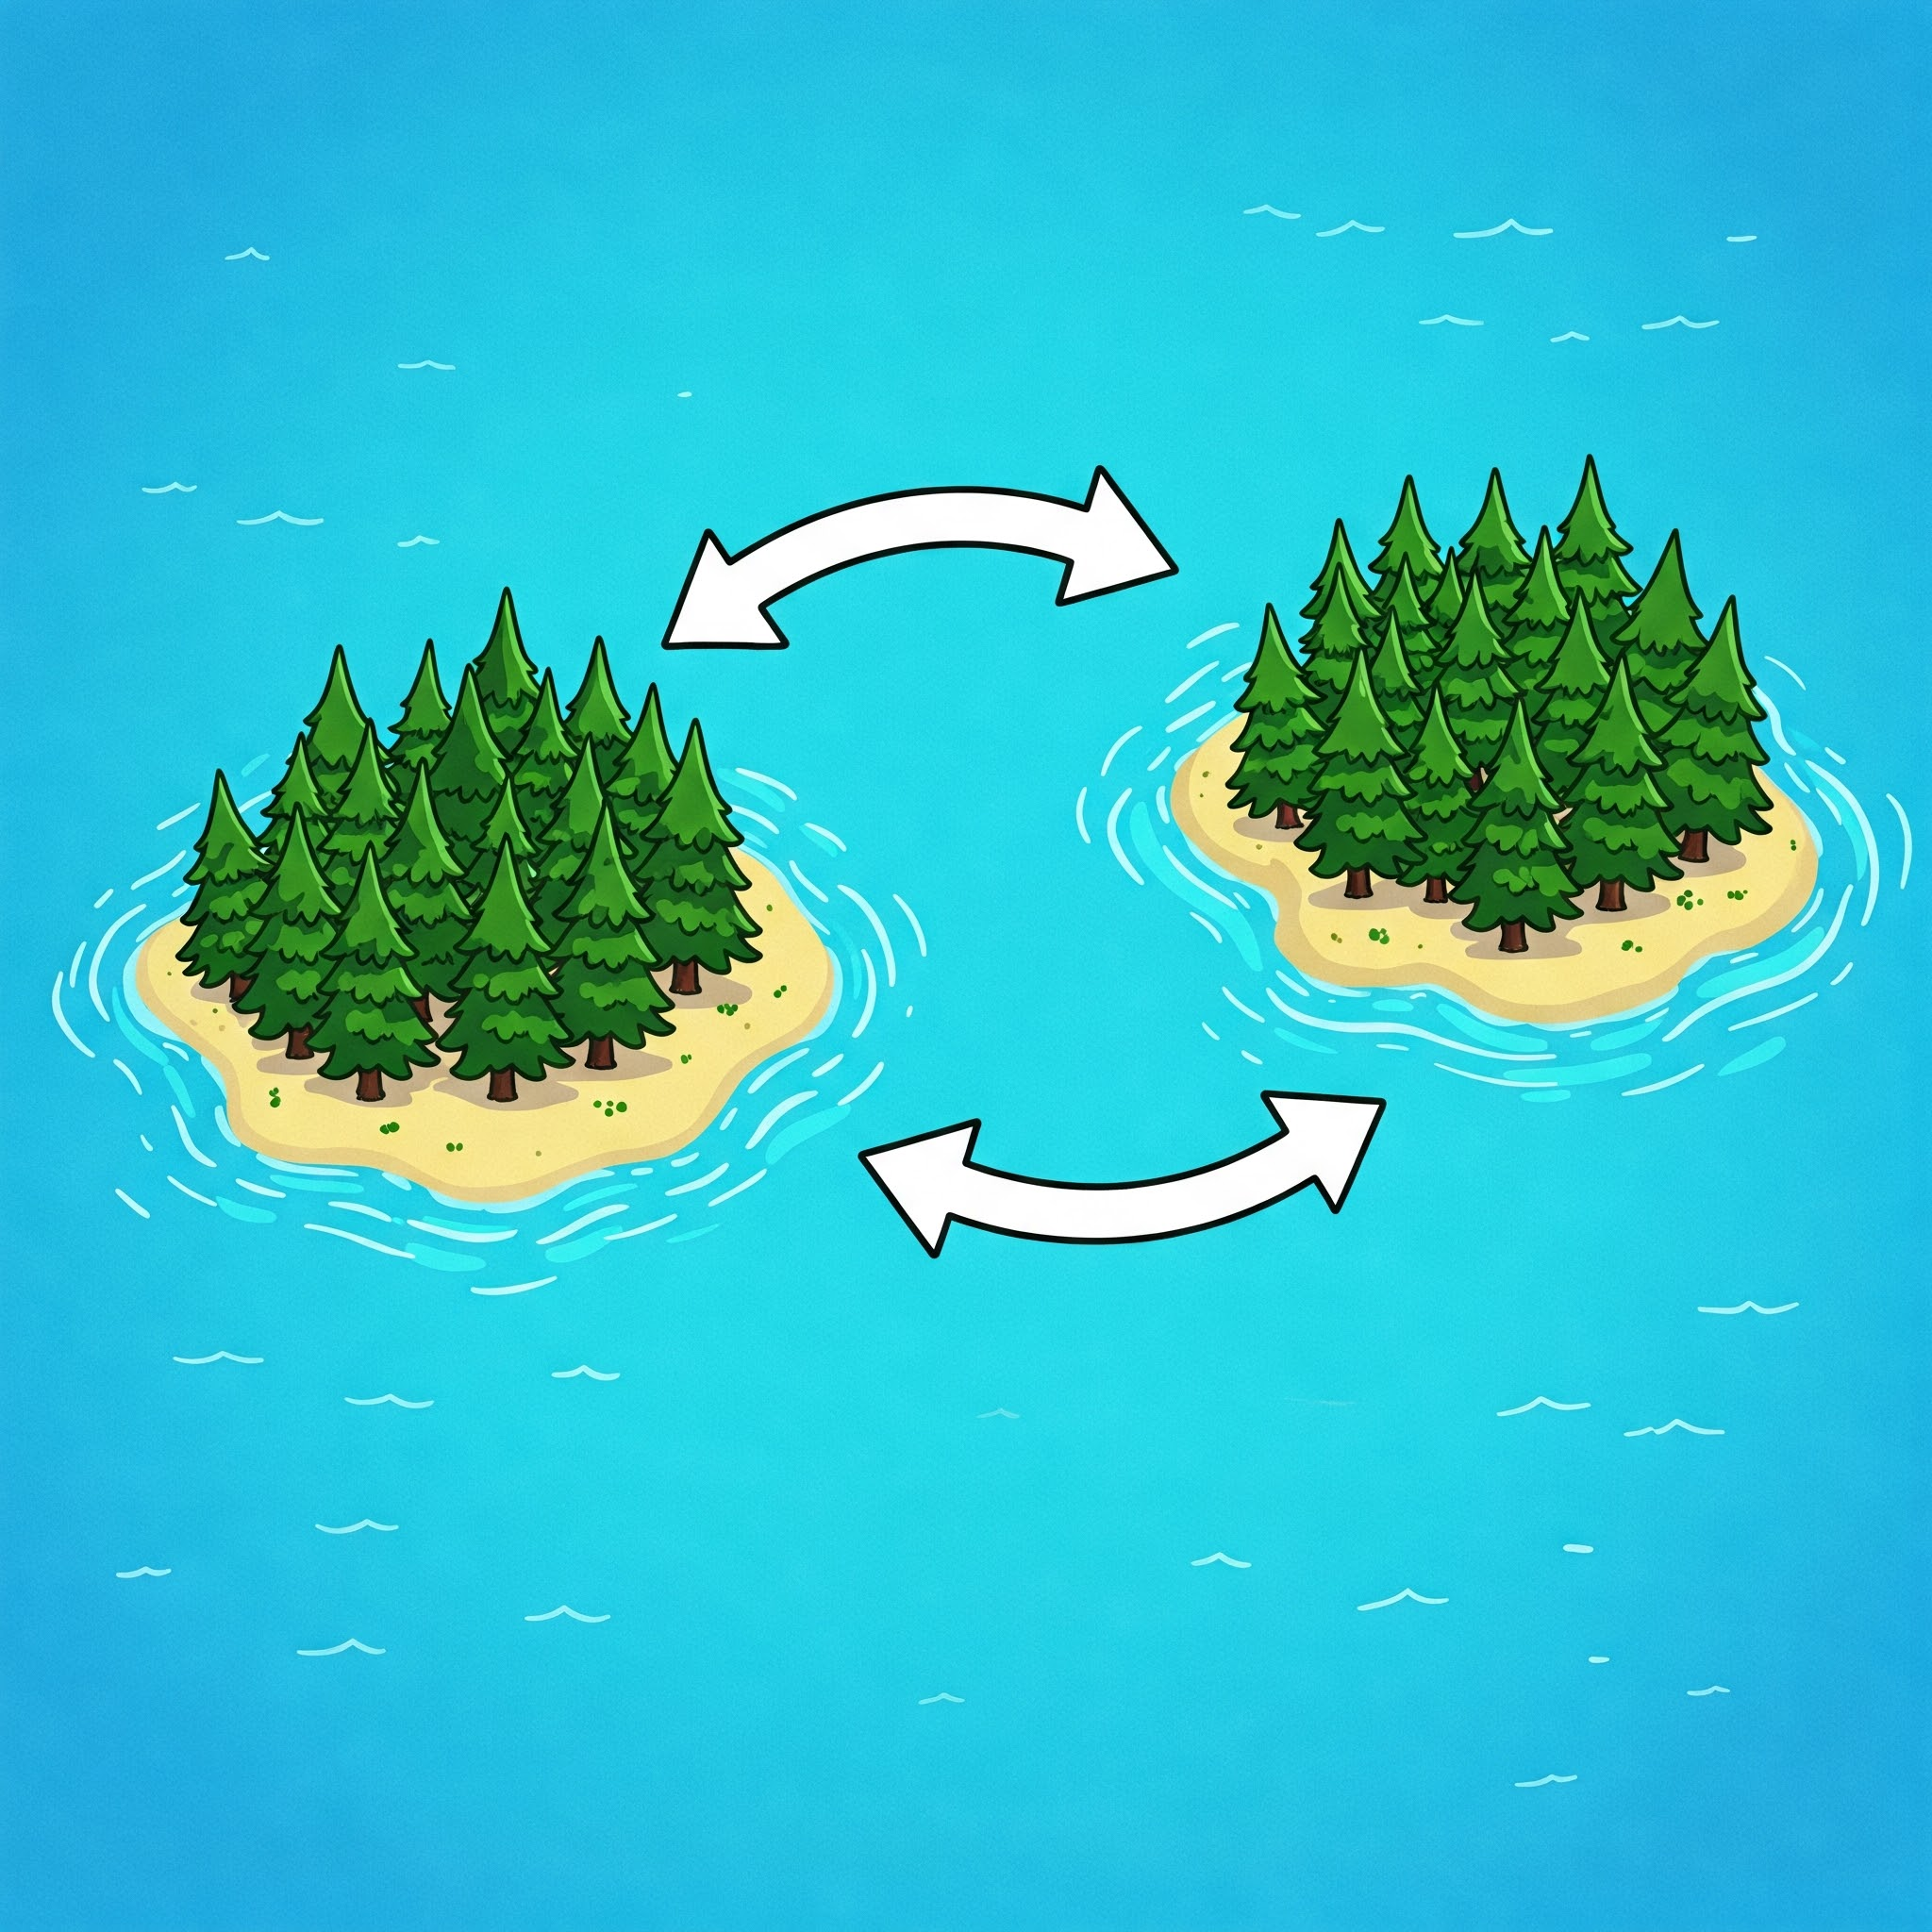
\includegraphics[keepaspectratio, width  = 0.7\textwidth]{img/treeIslands}
			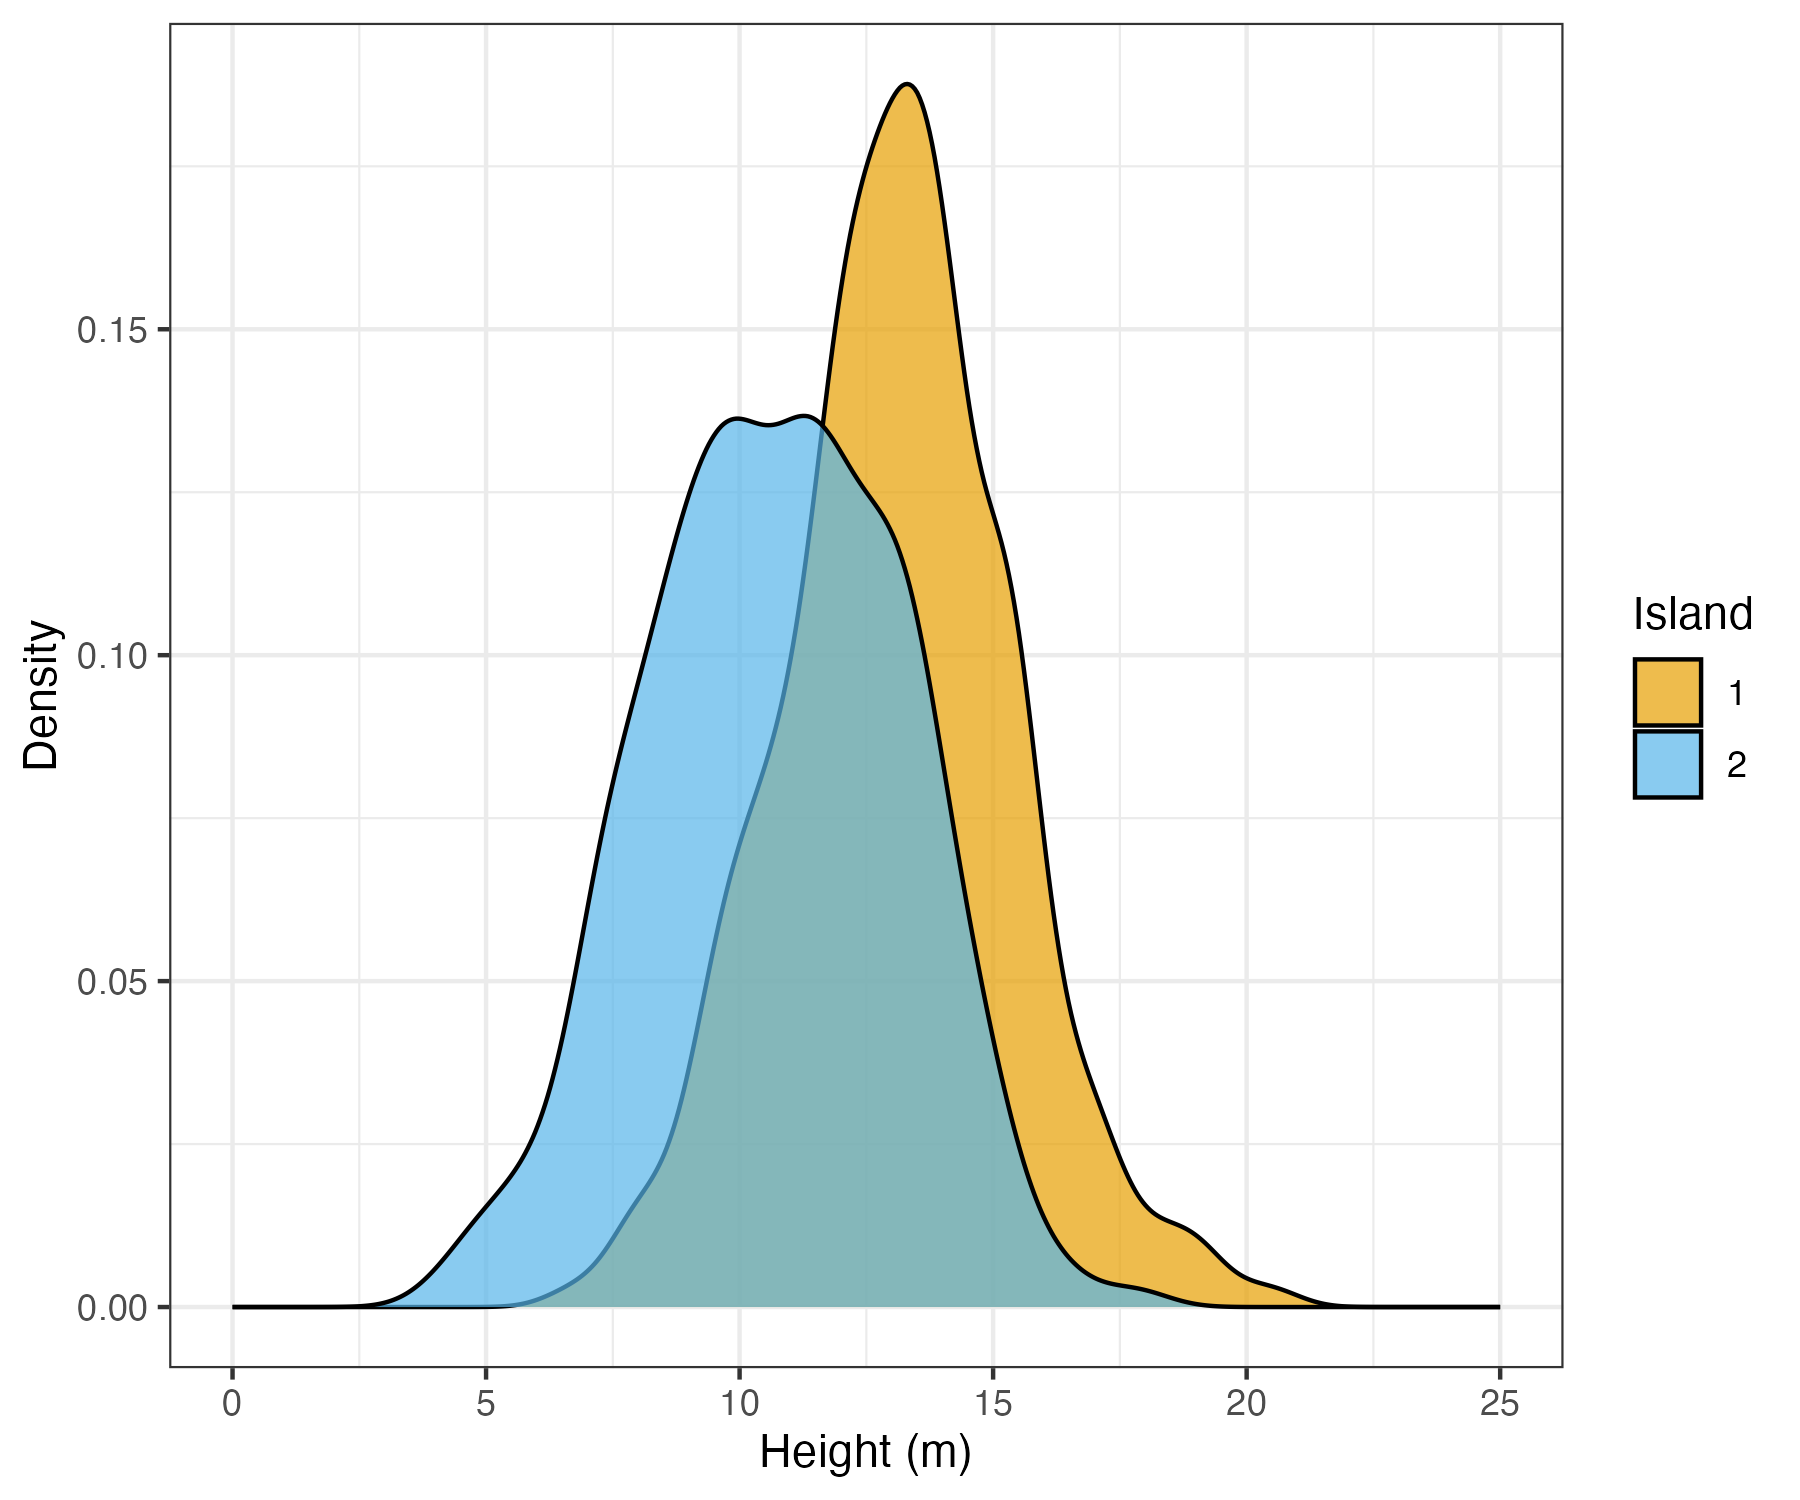
\includegraphics[keepaspectratio, width  = 0.9\textwidth]{img/treePhens.png}				
			
			
		\end{column}
		\begin{column}{0.4\textwidth}
			\begin{itemize}
				\item[-] In our model, trees are restricted to two distinct islands with a small amount of gene flow
				\item[-] We can factor the relationship among individuals into our statistical model 
				\item \scriptsize (\textit{there are a variety of ways to do this, but we won't get into the specifics today}) 
			\end{itemize}
		\end{column}
	\end{columns}

\end{frame}


\begin{frame}
	\frametitle{Genome-Wide Association Study}
	Now, let's look at each SNP across the whole genome 
	
	\includegraphics[keepaspectratio, width  = 0.95\textwidth]{img/corPlot_}				
	
	\blfootnote{We corrected for population structure using a matrix of relatedness among individuals (see Lecture 4.3)}
\end{frame}


\begin{frame}	
	\frametitle{Association Genetics Caveat: Multiple Testing}
\begin{itemize}	
\item In GWAS, we are conducting many tests (i.e. on each SNP) simultaneously
\end{itemize} \pause


\begin{columns}
	\begin{column}{0.5\textwidth}
		Let's do a simple experiment...\\
		\begin{itemize}
			\item[-] Draw 100 numbers at random between 0 and 1, call this $A$ \pause
			\item[-] Draw another 100 numbers at random between 0 and 1, call this $B$ \pause
			\item[-] Calculate the means of $A$ and $B$ \pause
			\item[-] What is the expected difference between $A$ and $B$? \pause
			\end{itemize}
		
		
	\end{column}
	\begin{column}{0.5\textwidth}
	\end{column}
\end{columns}





\end{frame}

\begin{frame}
		\frametitle{Genome-Wide Association Study - Redo}

Let's now correct for the issues we have identified so far...

\end{frame}




\end{document}


%%%
	\begin{columns}
	\begin{column}{0.5\textwidth}
	\end{column}
	\begin{column}{0.5\textwidth}
	\end{column}
\end{columns}



